In the previous chapter, we have seen how the many-body problem can be decoupled into an electronic problem given by Eq.\,\eqref{eq:Hsolution1}, which can be solved in the framework of DFT, and a nuclear problem given by Eq.\,\eqref{eq:chi2} that describes the dynamical properties of the nuclei. This was achieved by means of the Born-Oppenheimer approximation where electron-nucleus interactions beyond a parametric dependence on each other are neglected~\cite{BornOppenheimer}.

\newthought{We will now approach} the description of the nuclear dynamics from two sides: First, we treat the nuclei as \emph{classical} particles on the full, non-truncated Born-Oppenheimer potential. This will lead to the formulation of \emph{ab initio molecular dynamics} (aiMD). 
Second, we introduce the \emph{harmonic approximation} in which the nuclear Schr\"odinger equation is solved for an approximated potential.
As no electron will appear anymore, $N \equiv N_{\rm Nuc}$ will henceforth denote the number of nuclei in the system of interest, and we denote the Born-Oppenheimer potential simply as \emph{the} potential, $\mathcal V ({\bf R})$.

We begin by recalling the Schr\"odinger equation for the nuclear wavefunctions $\chi_s ({\bf R})$ initially defined in Eq.\,\eqref{eq:chi2},
\begin{align}
  \left( T^{\rm Nuc} + \mathcal V ({\bf R}) - E \right) \chi ({\bf R})
  = 0~,
  \label{eq:BOSE}
\end{align}
where
\begin{align}
  T^{\rm Nuc}
    = \sum_I \frac{- \hbar^2}{2 M_I} \frac{\partial^2}{\partial {\bf R}_I^2}~,
  \label{eq:Tnuc2}
\end{align}
is the nuclear kinetic-energy operator as before.


\section{Classical Limit}
The classical limit of the nuclear Schr\"odinger equation~\eqref{eq:BOSE} is usually performed by writing the nuclear wavefunction $\chi_s ({\bf R}, t)$ in terms of a real amplitude $A_s({\bf R}, t)$ and a \emph{classical action function} $S_s({\bf R}, t)$~\cite{Dirac1981,Landau2013,Marx2009}
\begin{align}
\chi_s({\bf R}, t) = A_s({\bf R}, t) \, {\rm e}^{\frac{\im}{\hbar} S_s({\bf R}, t)}~.
\label{eq:class.1}
\end{align}
The Schr\"odinger equation then yields a set of differential equations for $A_s$ and $S_s$ that, in the limit $\hbar \to 0$, go over to a \emph{Hamilton-Jacobi} equation for the action $S_s$,
\begin{align}
\frac{\partial S_s}{\partial t} + \mathcal H \left({\bf R}, {\bf P}\right)
= 0~,
\label{eq:HamiltonJacobi}
\end{align}
where ${\bf P} = ({\bf P}_1, \ldots) \equiv ({\bf \nabla}_1 S_s, \ldots)$ denotes the conjugate momenta and $\mathcal H$ is the \emph{classical} Hamilton function\footnote{We use the terms \emph{Hamilton function} and \emph{Hamiltonian} interchangeably in the following.} corresponding the to the operator in Eq.\,\eqref{eq:BOSE}, from which the equations of motion for the nuclei can be obtained:
\begin{align}
\dot{{\bf P}}_I 
= -\frac{\partial \mathcal H}{\partial {\bf R}_I}
\quad\implies\quad M_I \ddot{\bf R}_I
= -\frac{\partial \mathcal V}{\partial {\bf R}_I}~.
% \equiv - {\bf F}_I~.
\end{align}
The negative gradient of the Born-Oppenheimer potential, 
$-\partial \mathcal V / \partial {\bf R}_I$ is the force ${\bf F}_I$ acting on atom $I$ which can be obtained via the Hellmann-Feynmann theorem,~cf.~Sec.\,\ref{sec:HellmannFeynman}.

\newthought{An alternative viewpoint} that is more instructive can be taken by invoking the \emph{Ehrenfest theorem}~\cite{Ehrenfest1927,Basdevant2007}. The statement is that
\begin{align}
\frac{\d}{\d t} \left\langle {\bf P}_I \right\rangle_{\chi_s}
= \left\langle
- \frac{\partial \mathcal{V}}{\partial {\bf R}_I}
\right\rangle_{\chi_s}~,
\label{eq:ehrenfest.de1}
\end{align}
where $\langle \cdot \rangle_{\chi_s}$ denotes an expectation value taken with respect to the state $\chi_s$. This expression differs only slightly from the classical counterpart, which would read
\begin{align}
\frac{\d}{\d t} \left\langle {\bf P}_I \right\rangle
= \left.
- \frac{\partial \mathcal{V}}{\partial {\bf R}_I}
\right\vert_{{\bf R} = \langle {\bf R} \rangle}~.
\label{eq:ehrenfest.de2}
\end{align}
The difference comes from the fact that, in quantum mechanics, the expectation value of a function of an observable does not equal the function of its expectation. In mathematical terms, we have
\begin{align}
\delta f  \equiv 
f \bm ( \langle x \rangle \bm{)} 
- 
\bm{\langle} f (x) \bm{\rangle}
\neq 0
~,
\label{eq:ehrenfest.delta1}
\end{align}
where $x = {\bf R}_I$ denotes the space coordinate for notional simplicity, $f$ is some function of the observable $x$, and $\delta f$ measures the difference between the classical and the quantum expectation value. Ehrenfest's argument is that this difference becomes negligible when the state is sufficiently peaked around some value $x_0$. Expanding $f$ around the expectation value of $x$ denoted by $x_0 \equiv \langle x \rangle$, we have
\begin{align}
f(x) = f \bm ( \langle x \rangle \bm{)}  
+ (x - \langle x \rangle) \, f' \bm ( \langle x \rangle \bm{)}
+ \frac{1}{2} (x - \langle x \rangle)^2 \, f'' \bm ( \langle x \rangle \bm{)}
+ \cdots~.
\label{eq:ehrenfest.f2}
\end{align}
It follows that the $f'$ term vanishes when the expectation value is taken, and
\begin{align}
\langle f(x) \rangle 
= f \bm ( \langle x \rangle \bm{)}  
+ \frac{1}{2} \Delta x^2 f'' \bm ( \langle x \rangle \bm{)}
+ \cdots~,
\label{eq:ehrenfest.f3}
\end{align}
where $\Delta x^2 = \bm{\langle} (x - \langle x \rangle)^2 \bm{\rangle}$ measures the variance of the underlying distribution,~i.\,e.~the width of the wavepacket. The relative error between the classical and quantum expectation value is readily computed to be proportional to the variance $\Delta x^2$,
\begin{align}
\left\lvert \frac{\delta f}{f \bm ( \langle x \rangle \bm{)}} \right\rvert
= \frac{1}{2} \Delta x^2 \left\lvert \frac{f'' \bm ( \langle x \rangle \bm{)}}{f \bm ( \langle x \rangle \bm{)}} \right\rvert
+ \mathcal{O}(\Delta x^3)~.
\label{eq:ehrenfest.delta2}
\end{align}
This estimation holds in general for any observable $f$.
By crudely estimating the dimension of the wavepacket in terms of the thermal de Broglie-wavelength, we find
\begin{align}
\Delta x^2 
\sim \left( \frac{h}{P} \right)^2
\sim \frac{h^2}{MT}~,
\label{eq:ehrenfest:dimension}
\end{align}
where $h$ is Planck's constants, $M$ is the atomic mass, and $T$ is temperature. This estimate gives support to the intuitive assumption that we can expect the classical limit to work better the heavier the atoms and the higher the temperature.
Let us now set $f(x) \hat = -\partial \mathcal V / \partial {\bf R}_I$, then another important conclusion can be drawn from Eq.\,\eqref{eq:ehrenfest.delta2}: For a harmonic potential $\mathcal V ({\bf R}) = \mathcal V^{(2)} ({\bf R})$, where derivatives higher than second order vanish, the classical and quantum mechanical expectation values \emph{coincide}. The quantum mechanical expectation value of position will therefore evolve in the same time-periodic fashion as a classical particle in a harmonic well.

\REM{this approach can only be validated by computing observables and compare the results. One can safely say that this approach has been used successfully in a plethora of studies, while additional care must be taken at low temperature and/or systems with light atoms, especially hydrogen-bonded systems~\CITE{MD-Review?,MarklandCeriotti,Litman,pHexperiment}.}

\newpage

\section{Harmonic Approximation}
The Born-Oppenheimer potential $\mathcal V ({\bf R})$ appearing in Eq.\,\eqref{eq:BOSE} is an ordinary function of the\marginnote{Remember $N \equiv N_{\rm Nuc}$.} $3 N$ coordinates ${\bf R} = ({\bf R}_1, \ldots, {\bf R}_{N})$ and therefore can be expanded as a Taylor series in displacements ${\bf U} \equiv \Delta {\bf R}$ about a given configuration ${\bf R}^0$,~i.\,e.,
\begin{align}
\begin{split}
  \mathcal V ({\bf R} = {\bf R}^0 + {\bf U})
    = \mathcal V ({\bf R}^0)
    &+ \sum_{I, \alpha} 
      \left. \frac{\partial \mathcal V({\bf R})}{\partial R^\alpha_I} 
      \right\vert_{{\bf R}^0}
    \,U^\alpha_I
    \\
    &
    + \frac{1}{2}
    \sum_{\substack{I, J \\ \alpha, \beta}}
    \left.\frac{\partial^{2} \mathcal{V}(\mathbf{R})}{\partial R_{I}^{\alpha} \partial R_{J}^{\beta}}\right|_{\mathbf{R}^{0}}
    \, U_I^\alpha U_J^\beta
    \\
    &+\frac{1}{3!}\cdots ~,
\end{split}
\end{align}
where the expansion coefficients are called \emph{force constants}. In particular, we have the \emph{harmonic force constants}
\begin{align}
  % \Phi_{\alpha, \beta}^{I, J}
  \Phi_{I \alpha, J \beta}
  \equiv \left.\frac{\partial^{2} \mathcal{V}(\mathbf{R})}{\partial R_{I}^{\alpha} \partial R_{J}^{\beta}}\right|_{\mathbf{R}^{0}}~.
  \label{eq:FC2}
\end{align}
The harmonic approximation is typically used to assess dynamical properties of a system in some confined phase-space region close to a (local) minimum of the potential-energy surface. A local minimum configuration ${\bf R}^0$ is characterized by
\begin{align}
	\left. \frac{\partial V({\bf R})}{\partial R^\alpha_I} 
	\right\vert_{{\bf R}^0} 
		&~=~ 0 \quad\text{for all}\quad (I, \alpha),~\text{and} \\
	\sum_{\substack{I, J \\ \alpha, \beta}}
	% \Phi_{\alpha, \beta}^{I, J}
	\Phi_{I \alpha, J \beta}
	\, U_I^\alpha U_J^\beta
		&~>~ 0 \quad\text{for all possible}\quad \set{{\bf U}_I}~.
	\label{eq:ha.positive}
\end{align}
The condition in Eq.\,\eqref{eq:ha.positive} is satisfied when the harmonic force constants $\Phi_{I \alpha, J \beta}$ are positive-definite. It needs to be fulfilled to make the Hamiltonian bounded.

\newthought{We define \emph{mass-reduced coordinates}} for the displacements,
\begin{align}
	{\bf u}_I 
		&\equiv \sqrt{M_I} {\bf U}_I~, 
		\label{eq:uI} \\
	{\bf p}_I 
		&\equiv -\im \hbar \frac{\partial}{\partial {\bf u}_I}~,
		\label{eq:pI} \\
	% D_{\alpha, \beta}^{I, J}
	D_{I \alpha, J \beta}
		&\equiv \frac{1}{\sqrt{M_I M_J}} 
		%\Phi_{\alpha, \beta}^{I, J}
		\Phi_{I \alpha, J \beta}~,
		\label{eq:D}
\end{align}
where Eq.\,\eqref{eq:D} defines the \emph{dynamical matrix} $\rm D$.
Using these coordinates, the Hamiltonian assumes the form
\begin{align}
	\begin{split}
		\mathcal{H}({\bf p}, {\bf u})
			&= T^{\rm Nuc} ({\bf p}) + \mathcal{V}^{(2)} ({\bf u})\\
			&= \halb \sum_I {\bf p}_I^2 + 
				\halb \sum_{\substack{I, J \\ \alpha, \beta}}
					D_{I \alpha, J \beta}
					\, u_I^\alpha u_J^\beta~.
	\end{split}
	\label{eq:ha.H1}
\end{align}
\newthought{As required earlier}, the dynamical matrix $\rm D$ is a positive definite matrix. Furthermore, we see from Eq.\,\eqref{eq:FC2} that $\rm D$ is symmetric in the $3N$ coordinates $(I, \alpha)$,
\begin{align}
	D_{I \alpha, J \beta} = D_{J \beta, I \alpha}~.
	\label{eq:D.symmetric}
\end{align}
The eigenvalues of $\rm D$ will therefore be real and positive, and the eigenvectors will be real and orthogonal. We denote the eigenvalues as $\omega_s^2$ and the normalized eigenvectors as ${\bf e}_s$, where $s$ is the \emph{mode} label. $\omega_s$ will have the unit of a frequency and  will be called \emph{eigenfrequency} in the following. The dynamical matrix elements can be rewritten in therms of the eigenvectors and eigenvalues as
\begin{subequations}
\label{eq:D_IJ}
\begin{align}
	\sum_{J \beta}
		D_{I \alpha, J \beta} \, e_{s, J \beta} 
			&= \omega^2_s \, e_{s, I \alpha}~,~\text{or} 
			\label{eq:sum_D_IJ} \\
		D_{I \alpha, J \beta}
			&= \sum_s \omega^2_s \, e_{s, I \alpha} e_{s, J \beta}~.
			\label{eq:D_IJs}
\end{align}
\end{subequations}
Since the eigenvectors fulfill
\begin{align}
	\sum_{I \alpha} e_{s, I \alpha} e_{s', I \alpha} = \delta_{s s'}
	\quad \text{and} \quad
	\sum_{s} e_{s, I \alpha} e_{s, J \beta} = \delta_{IJ} \delta_{\alpha \beta}~,
	\label{eq:completeness.e_s}
\end{align}
we can rewrite the Hamiltonian in Eq.\,\eqref{eq:ha.H1} by using the dynamical matrix elements as defined in Eq.\,\eqref{eq:D_IJs}, so that
\begin{align}
	\mathcal{H}( {\bf p},  {\bf u})
		&= \halb \sum_s p_s^2 + 
		\halb \sum_{s} \omega_s^2	\, u_s^2~.
\label{eq:ha.H2}
\end{align}
Here, we implicitly defined the \emph{normal coordinates} $u_s$ and their conjugate momenta $p_s$,~i.\,e.,
\begin{align}
	u_s
		&= \sum_{I \alpha} e_{s, I \alpha} \, u_{I \alpha}~,
		\label{eq:u_s} \\
	p_s
		&= -\im \hbar \frac{\partial}{\partial u_s}~.
		\label{eq:p_s}
\end{align}
The Hamiltonian expressed in terms of the normal coordinates, Eq.\,\eqref{eq:ha.H2}, contains no cross-terms between different modes $s$ and $s'$. Rewritten in terms of this Hamiltonian, the wave equation \eqref{eq:BOSE} reads
\begin{align}
	\left\{
		\halb \sum_s p_s^2 + \halb \sum_{s} \omega_s^2	\, u_s^2 - E~.
	\right\} \chi ({\bf u})
	= 0
	\label{eq:ha.SE.2}
\end{align}
Since the Hamiltonian is a sum of terms, each depending on one coordinate only, the total nuclear wavefuntion $\chi$ can be separated into a product of wavefunctions for each mode,
\begin{align}
	\chi({\bf u}) = \prod_{s} \chi_s (u_s)~.
	\label{eq:ha.chi}
\end{align}
We end up with a set of $3N$ uncoupled equations, one for each mode $s$:
\begin{align}
	\left\{	\halb \left( p_s^2 + \omega_s u_s^2 \right)	- E_s	\right\} \chi_s (u_s)
		= 0~,
	\label{eq:ha.SE.single}
\end{align}
where the total energy of the nuclei is the sum of each mode contribution $E = \sum_s E_s$. Equation \eqref{eq:ha.SE.single} is the familiar equation for a harmonic oscillator of frequency $\omega_s$~\cite{Dirac1981}. Permissible solutions are labeled by the integer $n_s \in \mathds N_0$ and the eigenvalue $E_s$ depends on $n_s$ via
\begin{align}
	E_s(n_s) = \hbar \omega_s \left( n_s + \halb \right)~.
	\label{eq:E_s}
\end{align}
The state of the entire system is therefore specified by the $3N$ quantum numbers ${\bf n} = (n_1, \ldots, n_{3N})$, and the total energy of the system is
\begin{align}
	E ({\bf n}) = \sum_s \hbar \omega_s \left( n_s + \halb \right)~.
\end{align}
The thermodynamic properties of such a system of harmonic oscillators follow from this spectrum in straighforward fashion~\cite{BornHuang}.

This derivation is generally valid for a system of $N$ particles described by a potential-energy surface of which a (local) minimum ${\bf R}^0$, and the matrix of second derivatives at this configuration, $\Phi^{IJ}$, is known.

\subsection{Classical harmonic dynamics}

The classical dynamics generated by the harmonic Hamiltonian in Eq.\,\eqref{eq:ha.H2} is generated by the canonical equations of motion for the normal coordinates $\set{ u_s, p_s}$,
\begin{align}
	\dot{u}_s
		& = \frac{\partial \mathcal H}{\partial p_s}
			= p_s~,\quad\text{and}\quad
	\dot{p}_s
		 = - \frac{\partial \mathcal H}{\partial u_s}
			= - \omega^2_s u_s~.
\end{align}
The solution is given in terms of plane waves,
\begin{subequations}
\begin{align}
	u_s (t) 
		&= \phantom{\omega_s} \sqrt 2 A_s \sin (\omega_s t + \varphi_s)~,\\
	p_s (t) 
		&= \sqrt 2 \omega_s A_s \cos (\omega_s t + \varphi_s)~,
\end{align}
\end{subequations}
where $A_s$ and $\varphi_s$ are chosen based on the initial conditions. It can be beneficial to define the normal coordinates in terms of the complex amplitudes $a^{(\dagger)}_s$ ~,
\begin{subequations}
\begin{align}
	u_s (t) 
		&\equiv \frac{1}{\sqrt{2}} \left[ \D a_s (t) + \fD a_s (t) \right]~, \\
	p_s (t) 
		&\equiv \im \frac{\omega_s}{\sqrt{2}} \left[ \D a_s (t) - \fD a_s (t) \right]~,
\end{align}
\end{subequations}
with\marginnote{It follows $A_s = \lvert a_s (t) \rvert~.$}
\begin{subequations}
\begin{align}
	a_s (t) 
		& = {\rm e}^{- \im \omega_s t} a_s (0)~, \\
	a_s (0)
		& = A_s {\rm e}^{- \im \varphi_s}~.
\end{align}
\label{eq:a_s(t)}
\end{subequations}
The Hamiltonian in terms of the complex amplitudes $a^{(\dagger)}_s$ then reads\marginnote{The relation to quantum mechanics is achieved by replacing the complex numbers $a^{(\dagger)}_s$ with the operators $\sqrt{\frac{\hbar}{\omega_s}} \hat{a}^{(\dagger)}_s$ fulfilling the canonical commutation relations $$\left[ \fD{\hat{a}}_{\fP s}, \D{\hat a}_{s'} \right] = \delta_{ss'}~.$$}
\begin{align}
	\mathcal{H}(\b a, \D{\b a})
		&= \sum_s \omega^2_s \D a_s\fD  a_s~.
\end{align}

\subsection{Harmonic sampling}

\begin{align}
	\b U_I (t) 
		& = \frac{1}{\sqrt{M_I}} \sum_s \sqrt 2 A_s \b e_{sI} \sin (\omega_s t + \varphi_s)
\end{align}

by analogy with QM in thermal equilibrium\marginnote{Bose function ($\beta = 1 / k_{\mathrm{B}} T$): $$n_{\mathrm{B}}(\omega, T)=\frac{1}{\mathrm{e}^{\, \beta \hbar \omega}-1}~.$$}
\begin{align}
	E
		=\sum_{s} \hbar \omega_{s}\left(n_{\mathrm{B}}\left(\omega_{s}, T\right)+\frac{1}{2}\right)
\end{align}

\marginnote{In the classical limit $k_{\rm B} T \gg \hbar \omega_s$, this yields the equipartition +$E_s = 3 \kb T$.}
\begin{align}
	\braket{A_{s}^{2}}
		= \frac{\hbar}{\omega_{s}}\left(n_{\mathrm{B}}(\omega, T)+\frac{1}{2}\right)
		\underset{k_{\rm B} T \gg \hbar \omega_s}{\longrightarrow} \frac{k_{\rm B} T}{\omega_s^2}
\end{align}

\subsection{Mode projection}

Express amplitude $a_s (t)$ in terms of the atomic displacements $\set{\b U_I (t)}$ and velocities $\set{\dot{\b U}_I (t)}$ \TODO{Check units!}
The inverse relation between the amplitudes $a_s$ in terms of the conjugate variables $\set{u_s, p_s}$ is
\begin{align}
a_s (t) = u_s (t) + \frac{\im}{\omega_s} p_s (t)
\end{align}
with
\begin{subequations}
	\label{eq:mode.projection.u.p}
\begin{align}
	u_s (t) 
	    & = \sum_I \sqrt{M_I} \b e_{sI} \cdot \b U_I (t) \\
	p_s (t)
	    & = \sum_I \sqrt{M_I} \b e_{sI} \cdot \dot{\b U}_I (t) %\\
%	\implies
%	a_s (t) 
%	    &= \sum_I \sqrt{M_I} \b e_{sI} \cdot \left[ \b U_I(t) + \frac{\im}{\omega_s} \dot{\b U}_I (t) \right]
\end{align}
\end{subequations}



\section{Periodic Systems}
As already mentioned in Sec.~\ref{sec:theory.periodic.1}, the crystalline state is characterized by a periodic long-range order described the Bravais vectors ${\bf L} = L^i {\bf a}_i$, where $\set{{\bf a}_i}$ is the crystal basis and $L^i \in \mathds Z$.
We define this symmetry as follows:
Let ${\bf R}^0 = \set{{\bf R}_I^0}$ be the configuration of atoms in the local minimum of interest, and let ${\bf R}^{0 \prime} = \set{{\bf R}^{0 \prime}_{I}}$ denote the configuration obtained by moving all atoms by a Bravais vector ${\bf L}$,
\begin{align}
	{\bf R}^{0 \prime}_{I} = {\bf R}^0_{I} + {\bf L}~.
	\label{eq:RI'}
\end{align}
As a prerequisite for $\mathcal V ({\bf R})$ to be translationally invariant, we require that ${\bf R}^{0 \prime} = \set{{\bf R}^{0 \prime}_{I}}$ is a minimum configuration of the potential as well, \emph{and} there is a bijective permutation map $P_{\bf L}$ between the atomic positions ${\bf R}^{0 \prime}_{I}$ and ${\bf R}^{0}_{I'}$ which fulfills
\begin{align}
	P_{\bf L} : I \to I' \quad\text{such that}\quad
	{\bf R}^{0 \prime}_{I}
		= {\bf R}^{0}_{I'}~.
	\label{eq:translation.permutation}
\end{align}
This statement is equivalent to requiring that the configurations ${\bf R}^{0 \prime}_{I}$ and ${\bf R}^{0}_{I}$ are indistinguishable.\footnote{This requirement is obviously not fulfilled for molecules, where rigidly shifting all atoms can by no means induce a permutation map between atoms.} 
The final requirement for translational invariance of the potential is that the potential energy for \emph{any} configuration differing by a Bravais vector is unchanged:
\begin{align}
%	{\bf R}^{0 \prime}
%	= \set{{\bf R}_{I'}^0 }
%	&= {\bf R}^0 = \set{{\bf R}_{I}^0 }~,
%	\quad\text{and}
%	\label{eq:inv.R0} \\
	\mathcal{V} \left( {\bf R}' = \set{{\bf R}_{I} + {\bf L}} \right)
	&= \mathcal{V}({\bf R} = \set{{\bf R}_{I}} ) 
	\quad\text{for all}\quad {\bf L} = L^i {\bf a}_i~.
	\label{eq:inv.V}
\end{align}
This effectively corresponds to a permutation of the displacements of the atoms, $U_I \to U_{I'}$ according to $P_{\bf L}$. Figure\,\ref{fig:translation.permutation} shows a one-dimensional depiction of the relation between discrete translation by Bravais vectors and the permutation map.
\begin{marginfigure}
	\centering
	% 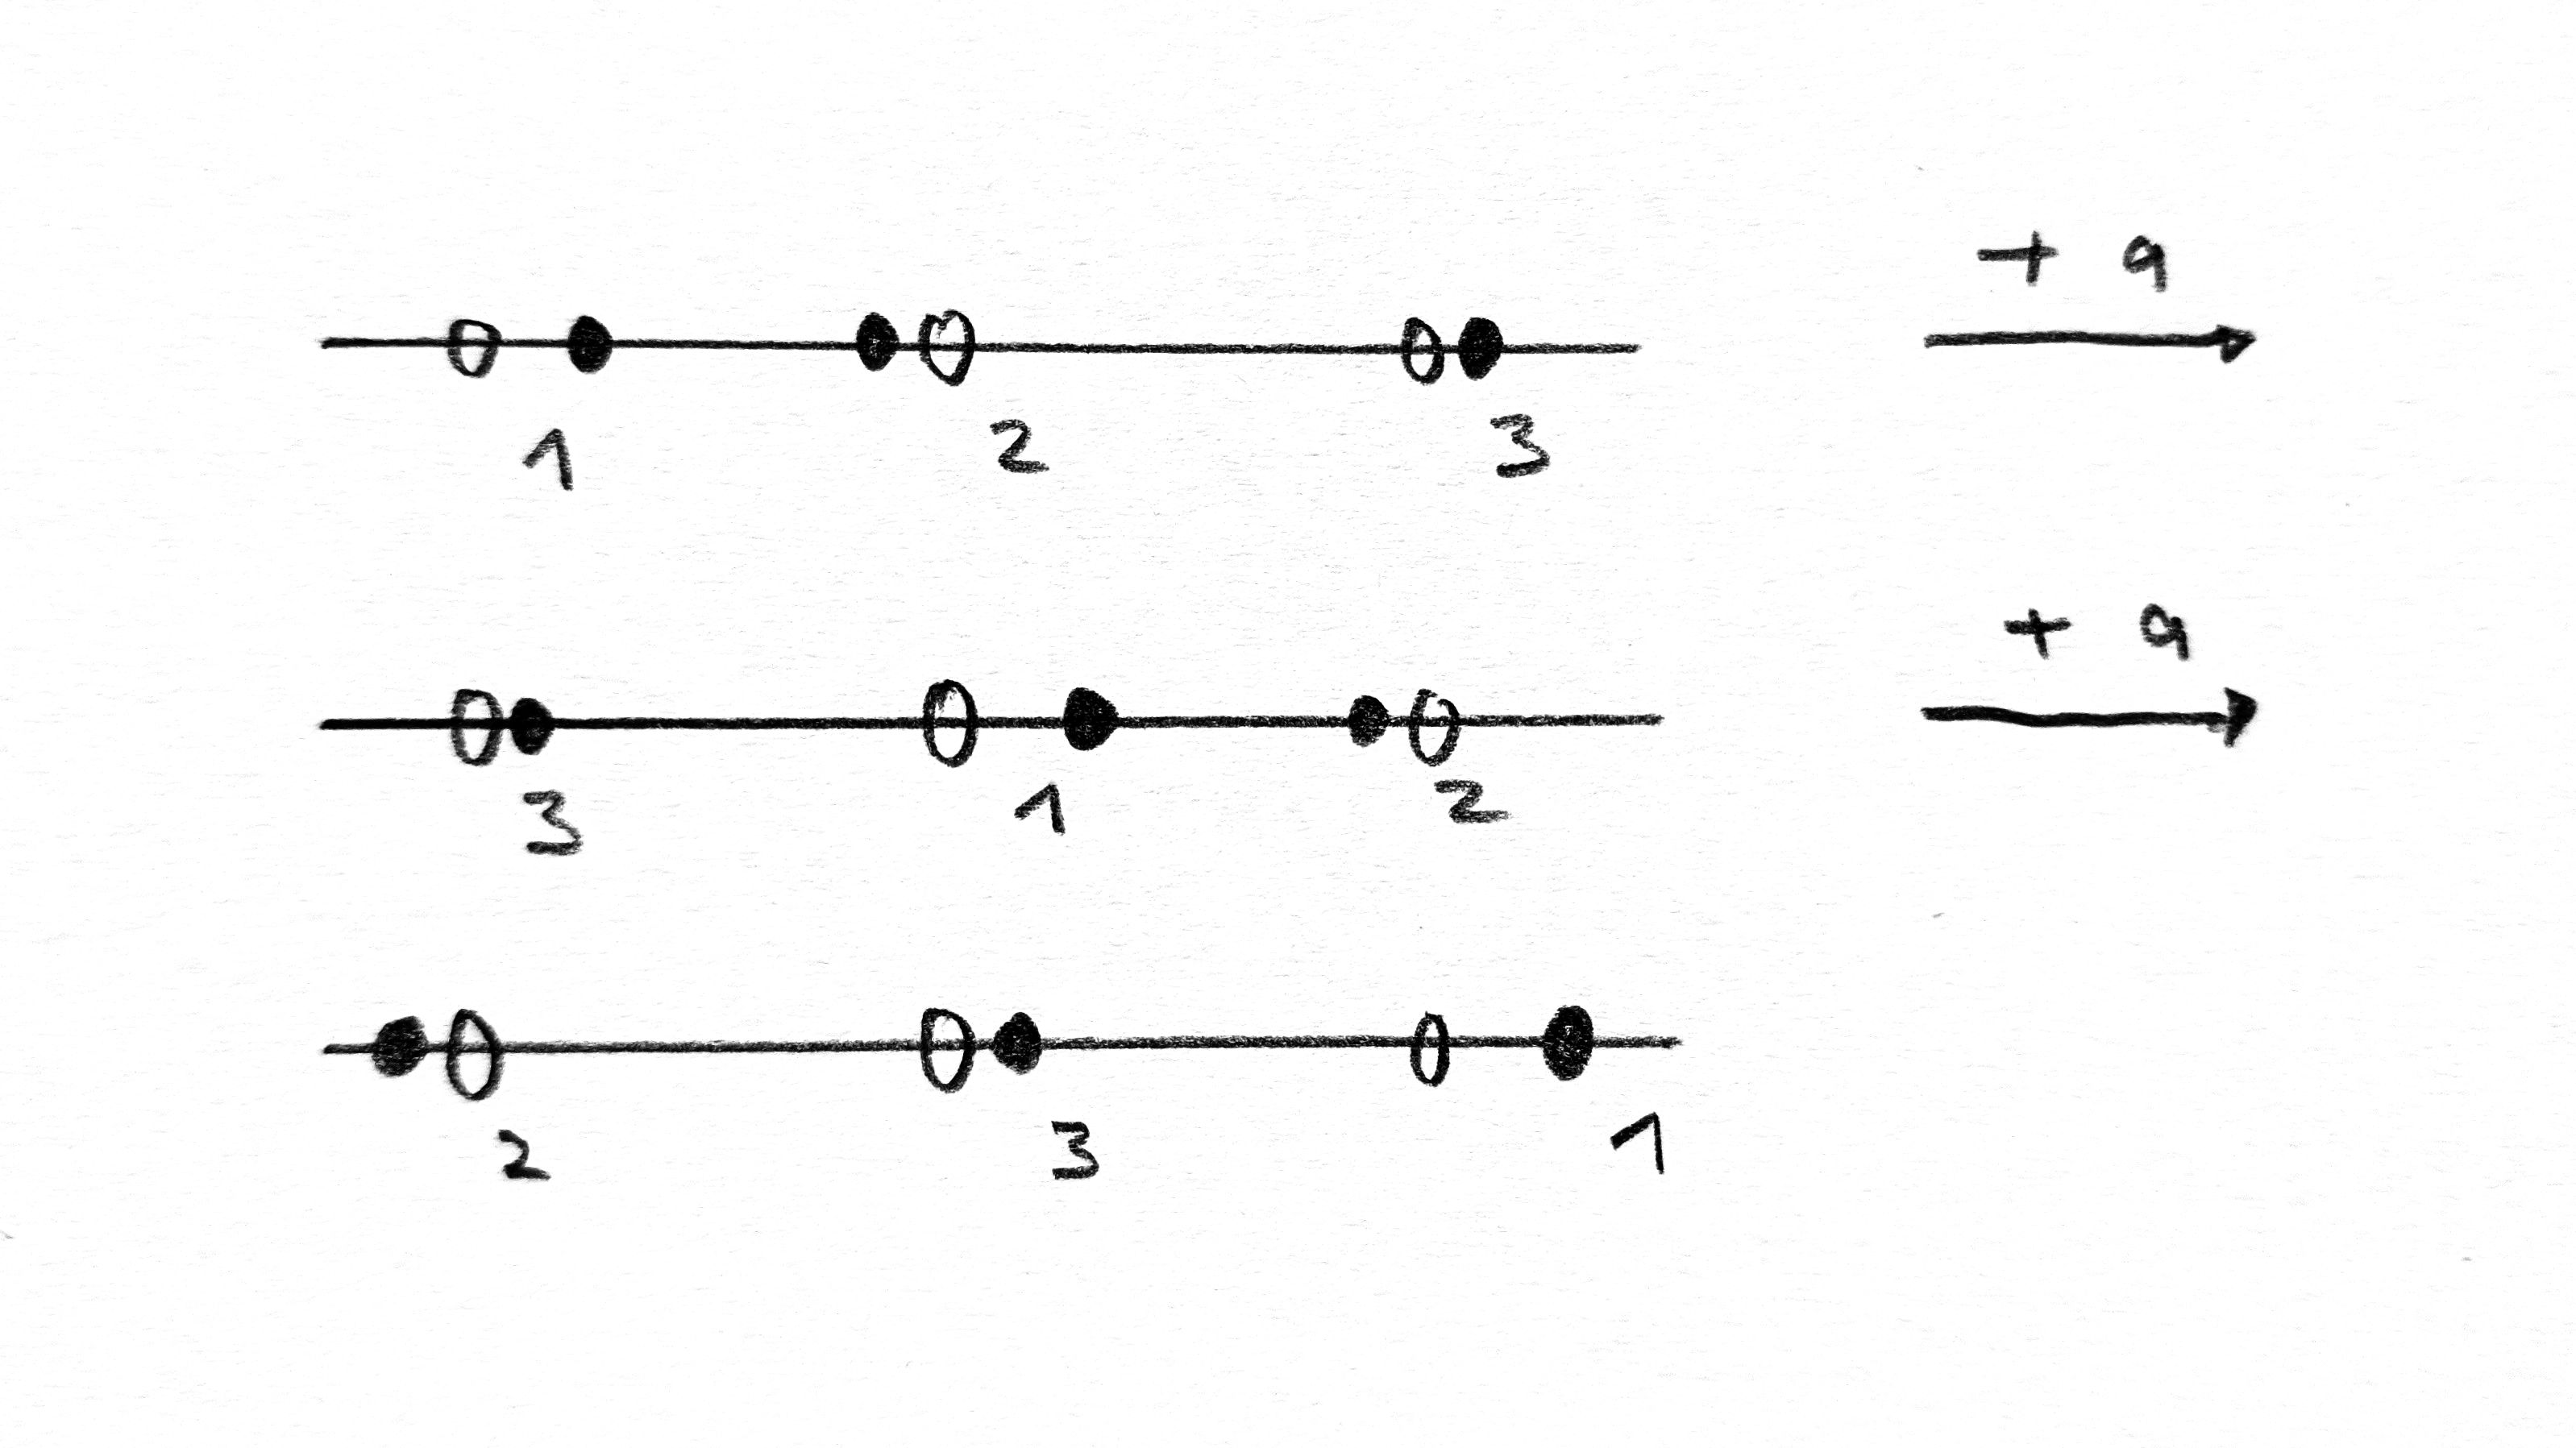
\includegraphics[width=.68\textwidth]{./sketches/permutation1.jpg}
	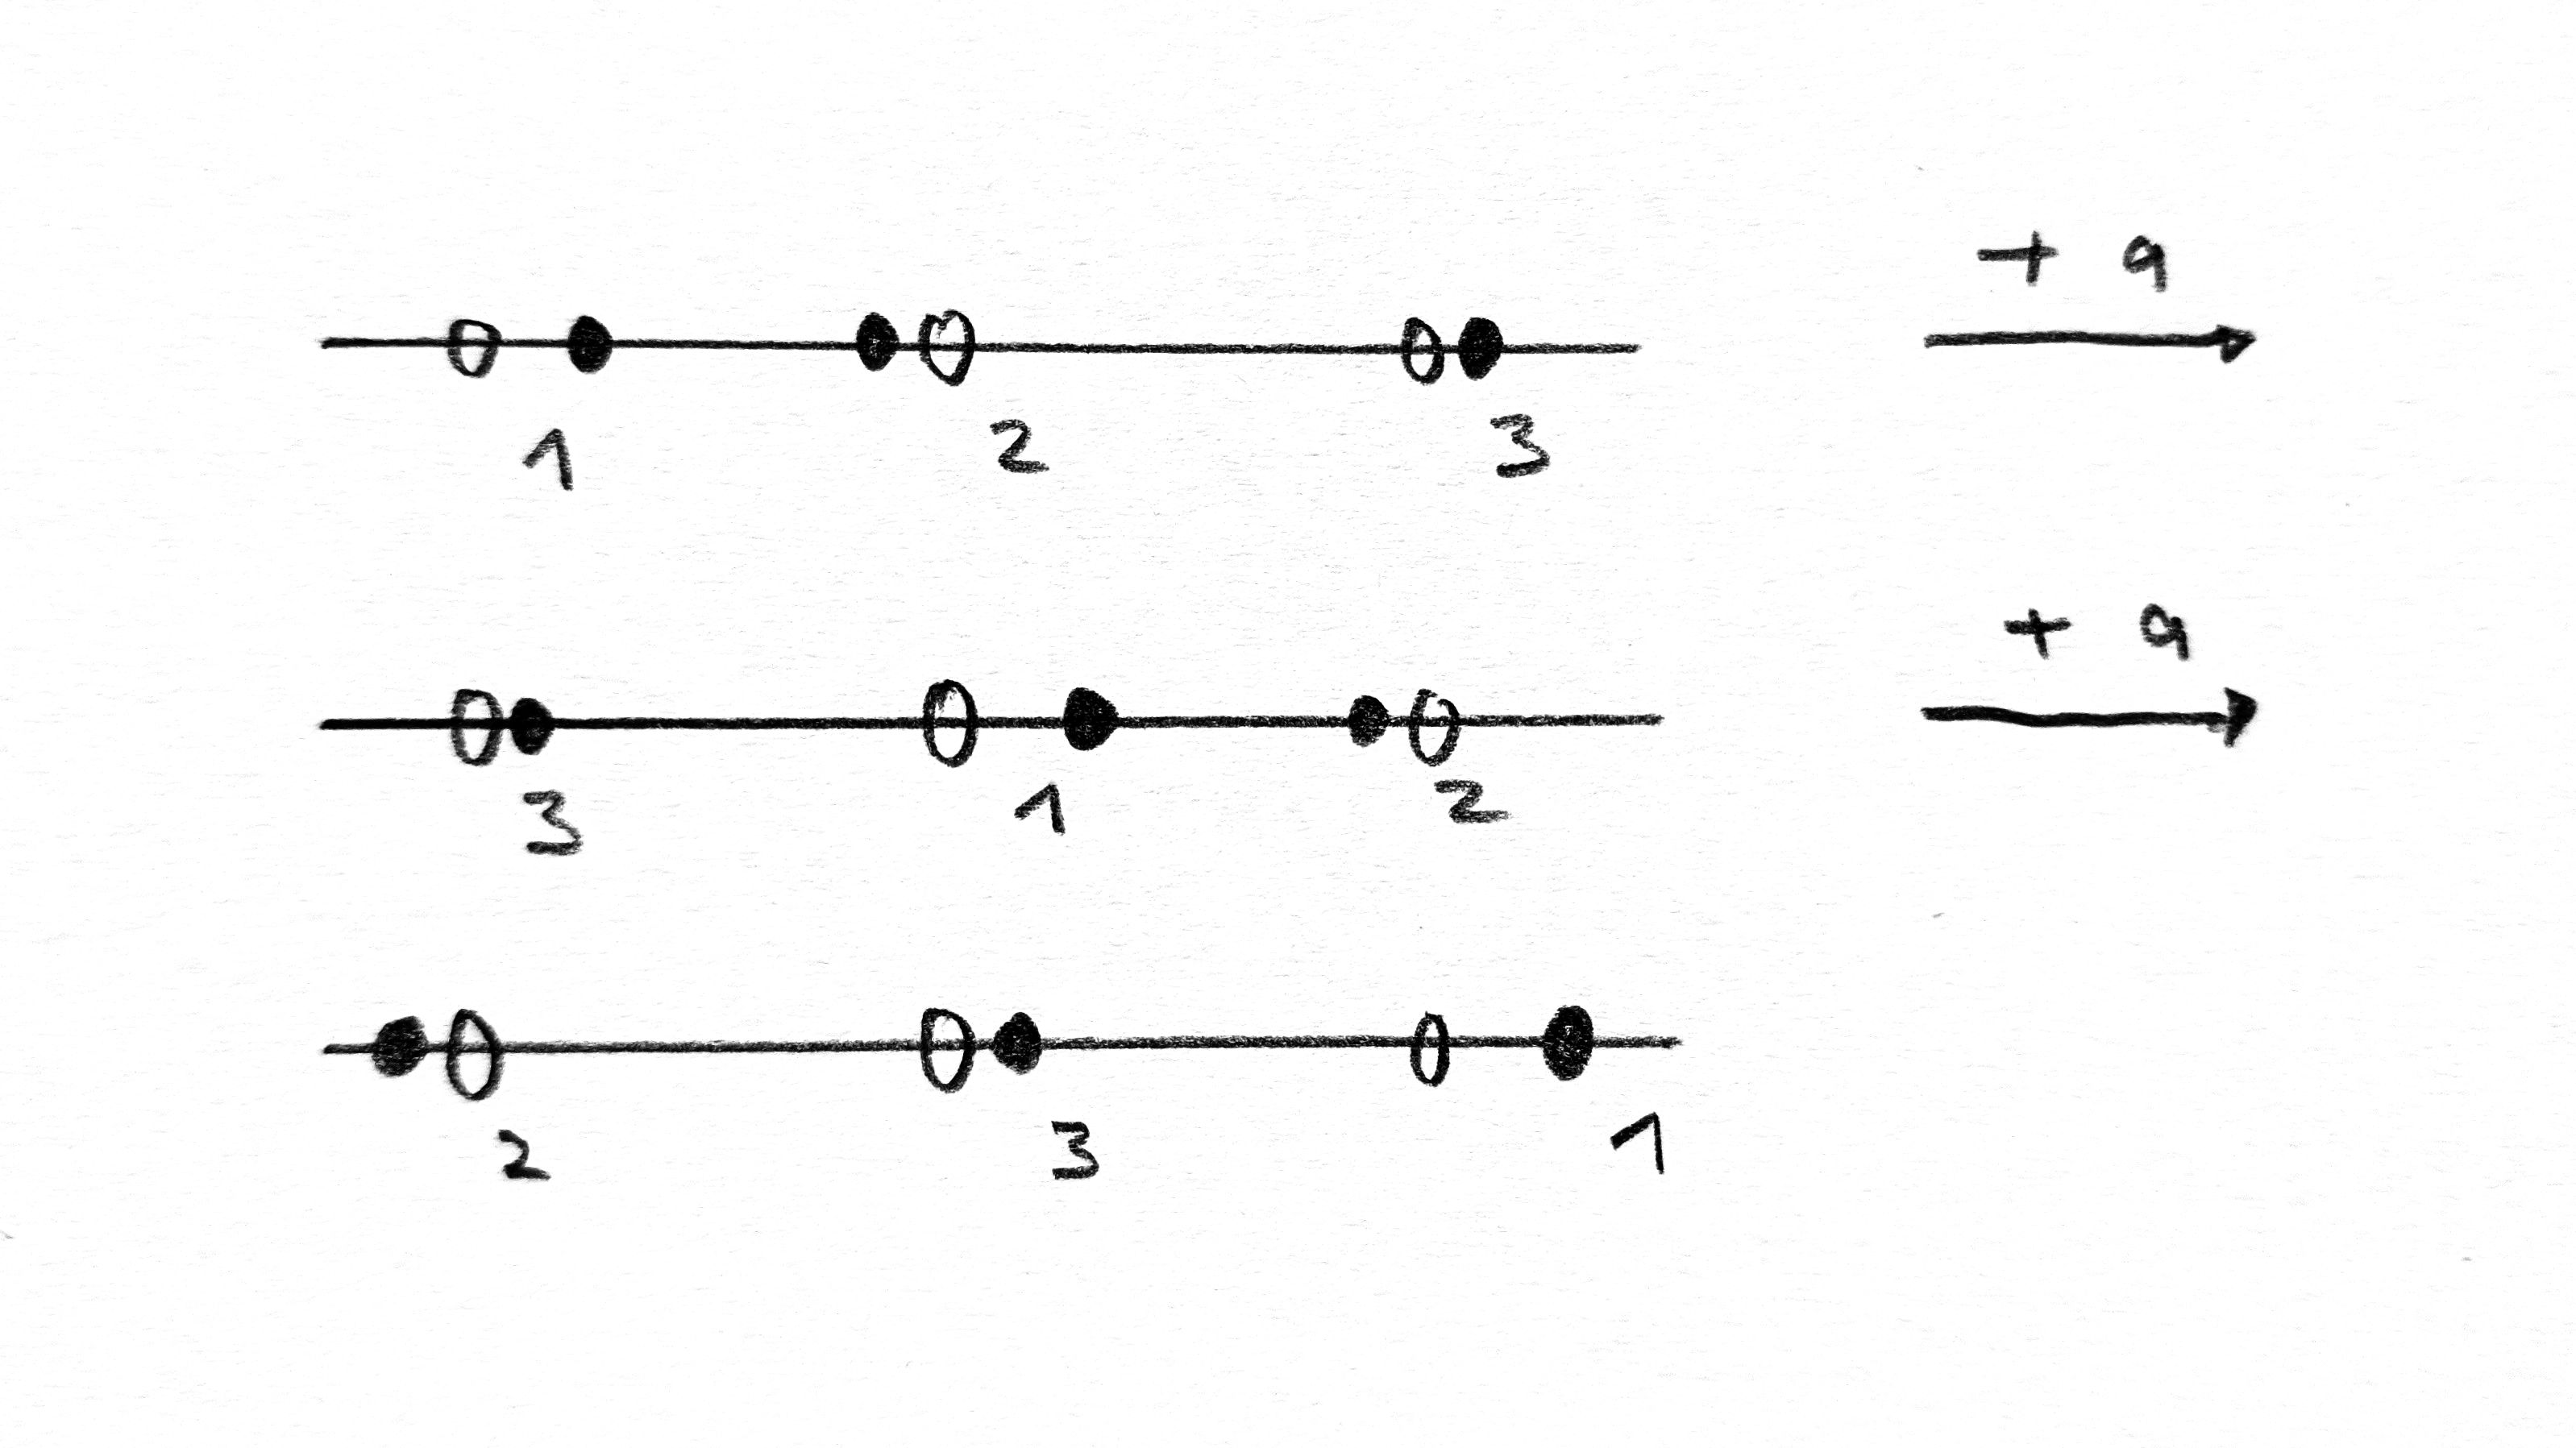
\includegraphics[width=\textwidth]{./sketches/permutation1.jpg}
	\caption{A linear chain with three atoms (bullets) displaced from their equilibrium position (open circels). With periodic boundary conditions, the consecutive translation by a lattice vector $a$ induces a permutation of the atoms,~i.\,e.,~$(1, 2 , 3) \to (3, 1, 2) \to (2, 3, 1)$.}
	\label{fig:translation.permutation}
\end{marginfigure}

We can draw two important conclusions from Eq.\,\eqref{eq:translation.permutation} and \eqref{eq:inv.V}. First, the existence of the map $P_{\bf L}$ enables us to write every atomic coordinate ${\bf R}_I$ as
\begin{align}
	{\bf R}_I \equiv {\bf R}_{i {\bf L}} 
		= {\bf R}^0_{i \b L} + {\bf U}_{i {\bf L}}
		= {\bf R}^0_i + {\bf L} + {\bf U}_{i {\bf L}}~,
	\label{eq:R_iL}
\end{align}
where ${\bf R}^0_i$ labels the position of an equivalent reference atom in the unit cell, ${\bf U}_{i {\bf L}}$ is the displacement of the atom from its equilibrium position, and $\bf L$ is a Bravais vector as before.
We can therefore split the index $I$ into a tuple $I = (i, {\bf L})$,~i.\,e.,~unit cell and lattice point labels.

Second, the harmonic force constants $\Phi_{I \alpha, J \beta}$ can be written as $\Phi_{i {\bf L} \alpha, j {\bf K} \beta}$~, where $\bf L$ and $\b K$ are the Bravais vectors belonging to $I$ and $J$, respectively. From the translational invariance of the potential, Eq.\,\eqref{eq:inv.V}, we see that the force constants have to fulfill
\begin{align}
	\Phi_{i {\bf L} + \b M \alpha, j {\bf K} + \b M \beta} 
		= \Phi_{i {\bf L} \alpha, j {\bf K} \beta}~,
	\label{eq:fc.sym.1}
\end{align}
where $\b M$ again denotes an arbitrary Bravais vector. Using this translational invariance, we can Fourier transform the dynamical matrix defined in Eq.\,\eqref{eq:D},
\begin{align}
	{D}_{i \alpha, j \beta} (\b q) 
		= \sum_{\b L} {\rm e}^{- \im \b q \cdot \b L} {D}_{i \b 0 \alpha, j \b L \beta}
	\label{eq:D(q)}
\end{align}
where we restrict the values of $\b q$ to reside in the first Brillouin zone, thereby transforming the $3N \times 3N$ matrix ${\rm D}_{IJ}$ to one $3n \times 3n$ matrix ${\rm D}_{ij} (\bf q)$ for each~$\b q$, where $n$ is the number of atoms in the primitive unit cell.

\subsection{Cyclic Boundary Conditions and Supercell Approximation}
In the previous section, we did not specify the system beyond requiring periodic boundary conditions, and implicitly assumed an infinite crystal in the limit $N \to \infty$ without boundaries. In practice we introduce Born-von Karman cyclic boundary conditions~\cite{born2013atomtheorie}, as already done in Sec.\,\ref{sec:theory.periodic.1} for the description of electronic states, but reintroduce them here in a slightly more general fashion.

\newthought{We define the boundary conditions} for the nuclear problem such that
\begin{align}
	\b R_I + S^i \b A_i = \b R_I \quad\text{for}\quad S^i \in \mathds{Z}~,
	\label{eq:sc.1}
\end{align}
where each ${\bf A}_i$ is a linear combination of the primitive basis vectors $\set{{\bf a}_i}$,
\begin{align}
{\bf A}_i = {\rm M}_{ij}^{\rm sc} {\bf a}_j\quad\text{with } {\rm M}_{ij}^{\rm sc} \in \mathds Z~,
\end{align}
and $\rm M^{\rm sc}$ is a non-singular matrix with integer elements. The space spanned by the $\set{{\bf A}_i}$ is parallelepiped of volume $V_{\rm sc} = N_{\rm sc} \, {\bf a}_1 \cdot ({\bf a}_2 \times {\bf a}_3)$, where $N_{\rm sc} = \det {\rm M}^{\rm sc}$ is the number of unit cells that fit into the enlarged cell, and $V_{\rm uc} = {\bf a}_1 \cdot ({\bf a}_2 \times {\bf a}_3)$ is the unit cell volume. This cell is therefore called \emph{supercell} and we define it such that its midpoint is located at the origin,~i.\,e.,~
\begin{align}
	\mathds V_{\rm sc}
		&= \set{{\bf X} = X^i {\bf A}_i : X^i \in {[-0.5, 0.5)_{\mathds R}}}~.
	\label{eq:supercell}
\end{align}
We therefore denote the matrix ${\rm M}^{\rm sc}$ as the \emph{supercell matrix}.
The vectors \mbox{$\b S = S^i \b A_i$} are the equivalent of the Bravais vectors $\b L$ in a superlattice described by $\set{ \b A_i }$ instead of $\set{ \b a_i}$.
The ideal, infinite crystal is obtained in the limit $N_{\rm sc} \rightarrow \infty$.
From Eq.\,\eqref{eq:sc.1} we see that the force constants become periodic functions in the superlattice,
\begin{align}
	\Phi_{i {\bf L} \alpha, j {\bf K} + \b S \beta} 
		= \Phi_{i {\bf L} \alpha, j {\bf K} \beta} \quad\text{for all}\quad \b S = S^i \b A_i~,
	\label{eq:fc.sym.2}
\end{align}
so that the dynamical matrix in Eq.\,\eqref{eq:D(q)} can be written as a sum over lattice points that are contained in the supercell only,
%\begin{align}
%	{\rm D}_{i \alpha, j \beta} (\b q) 
%		&= \sum_{\b L \in \mathds V_{\rm sc}} 
%			\left( 
%				{\rm e}^{- \im \b q \cdot \b L} {\rm D}_{i \b 0 \alpha, j \b L \beta}
%			+ \sum_{\b S \neq \b 0} {\rm e}^{- \im \b q \cdot (\b L + \b S)} {\rm D}_{i \b 0 \alpha, j \b L \beta}
%			\right)~.
%	\label{eq:D^S(q).1}
%\end{align}
\begin{align}
	{D}_{i \alpha, j \beta} (\b q_{\bf m}) 	
		&= %\frac{N}{N_{\rm sc}} 
	\sum_{\b L \in \mathds V_{\rm sc}} {\rm e}^{- \im \b q_{\bf m} \cdot \b L} {D}_{i \b 0 \alpha, j \b L \beta}~,
	\label{eq:D^S(q).2}
\end{align}
for $\b q_{\b m}$ that fulfill
\begin{align}
	{\bf q_{\b m}} \cdot {\bf A}_i	= 2 \pi m_i \quad\text{with}\quad m_i \in \mathds Z~.
	\label{eq:q.commensurate}
\end{align}
%the summands in the second sum of Eq.\,\eqref{eq:D^S(q).1} interfere constructively and yield a factor $\sum_{\b S}' = N / N_{\rm sc} - 1$. For all other $\b q$, the entire summand becomes negligible in the limit $N \to \infty$ when normalized to the supercell volume.
The $\b q_{\b m}$ that fulfill Eq.\,\eqref{eq:q.commensurate} are called \emph{commensurate} $\b q$-points, as they represent wave numbers that fit into the supercell.
In total there are $N_{\rm sc}$ non-equivalent values of $\bf q_{\b m}$ labelled by ${\bf m} = (m_1, m_2, m_3)$ that can be expressed in terms of the lattice vectors of the reciprocal supercell,
\begin{align}
{\bf B}^i 
= 2 \pi \varepsilon^{ijk} \frac{{\bf A}_j \times {\bf A}_k}{{\bf A}_1 \cdot ({\bf A}_2 \times {\bf A}_3)} ~,
%\label{eq:dft.Bloch.bi}
\end{align}
where $\varepsilon^{ijk}$ denotes the Levi-Civita symbol enforcing the correct ordering of $ijk$. The complete set of $\bf q$-values is
\begin{align}
{\bf q}_{\bf m} 
= \sum_{i=1}^3 m_i {\bf B}^i~,
\label{eq:q_m}
\end{align}
with $m_i \in \mathds Z$ such that $\b q_{\bf m}$ is an element of the first Brillouin zone of the direct lattice.
%For the set of commensurate $\b q$-points, the dynamical matrix is therefore given by
%\begin{align}
%{\rm D}_{i \alpha, j \beta} (\b q_{\bf m}) 	
%	&= %\frac{N}{N_{\rm sc}} 
%	\sum_{\b L \in \mathds V_{\rm sc}} {\rm e}^{- \im \b q_{\bf m} \cdot \b L} {\rm D}_{i \b 0 \alpha, j \b L \beta}~.
%	\label{eq:D^S(q).2}
%\end{align}


\subsection{Interpolation to non-commensurate q-points}
The definition of the dynamical matrix in Eq.\,\eqref{eq:D^S(q).2} was formulated for commensurate $\b q$-points $\set{\b q_{\b m}}$,~i.\,e.,~those given in terms of Eq.\,\eqref{eq:q_m}. Evaluating this expression at a non-commensurate value of $\b q$ will, in general, yield a non-hermitian matrix which cannot be used to extract physically sound information about the system. To obtain an \emph{approximated} dynamical matrix at any other, non-commensurate value of $\b q$ within the Brillouin zone, we define an \emph{extended supercell}, 
\begin{align}
	\mathds V_{\rm sc}^{\rm ext}
		&= \set{{\bf X} = X^i {\bf A}_i : X^i \in {[-0.5, 0.5 \boldsymbol{]}_{\mathds R}}}~,
	\label{eq:supercell.extended}
\end{align}
which also contains the lattice points at the positive boundary of the supercell as depicted by open circles in Fig.\,\ref{fig:sketch_supercells}.
\begin{marginfigure}[-6cm]
	\centering
	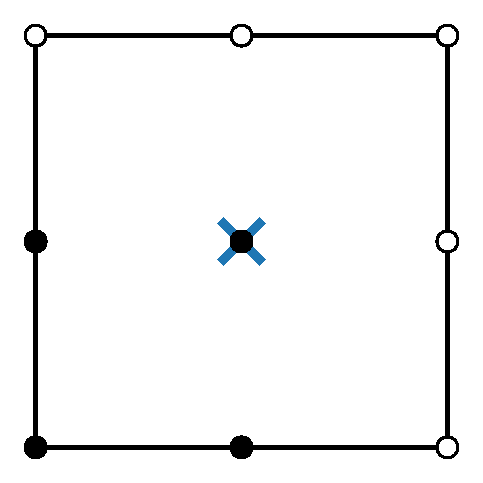
\includegraphics[width=.8\textwidth]{./sketches/2_sc.pdf}
	\hfill
	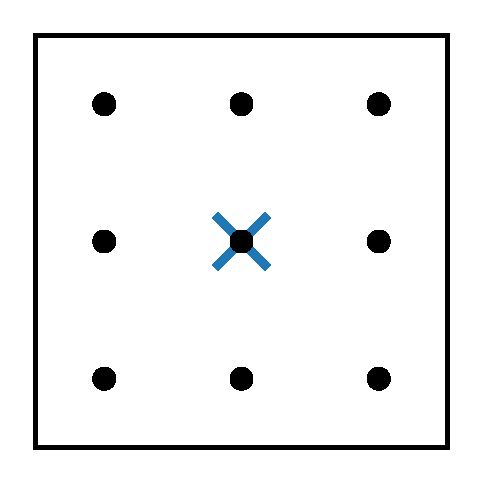
\includegraphics[width=.8\textwidth]{./sketches/3_sc.pdf}
	\hfill
	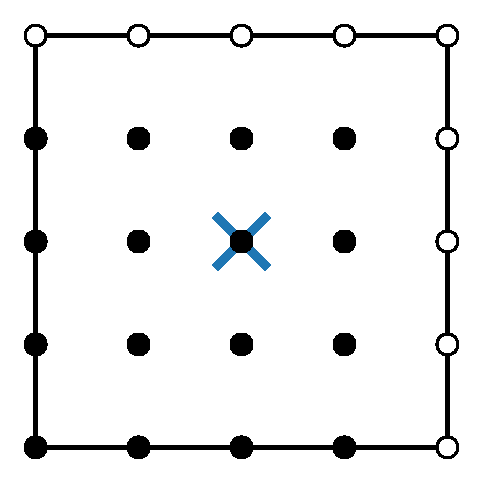
\includegraphics[width=.8\textwidth]{./sketches/4_sc.pdf}
	\caption{Depiction of square supercells with lattice points in the range $[-0.5 A, 0.5 A)$ (bullets $\bullet$), and extended lattice points at the supercell boundary (empty bullets $\circ$), where $A$ is the edge length of the supercell. Blue arrows denote the unit cell vectors, black arrows denote the supercell vectors.}
	\label{fig:sketch_supercells}
\end{marginfigure}
These lattice points are included in the Fourier series with an appropriate weight $w_{\b L}$ that accounts for double counting of lattice points that are separated by a linear combination of supercell lattice vectors~\cite{Parlinski1997}. Furthermore, we use a minimal image convention (MIC) between the atoms $(i, \b 0)$ and $(j, \b L)$: For each pair, we use an equivalent lattice point $\b L'$ within the extended supercell which depends on $(i, j, \b L)$ such that
\begin{align}
	- \b R_{i \b 0 } + \b R_{j \b 0} + \b L' \in \mathds V_{\rm sc}^{\rm ext}~.
	\label{eq:L'}
\end{align}
In total we define\marginnote{The dynamical matrix elements defined by Eq.\,\eqref{eq:D_Parlinski} differ from the ones found in Ref.~\cite{Parlinski1997} by a phase factor ${\rm e}^{\im \b q \cdot (\b R_i^0 - \b R_j^0)}$. The phase factor however does not affect the eigenfrequencies. It typically arises when the discussion is performed from a lattice-wave ansatz to solve the equations of motion~\cite[p. 298]{BornHuang} \TODO{Makes sense to include because harmonic heat flux becomes easier}}
\begin{align}
	{D}_{i \alpha, j \beta} (\b q) 	
		&= %\frac{N}{N_{\rm sc}} 
		\sum_{\b L \in \mathds V_{\rm sc}^{\rm ext}} 
			w_{\b L}
		{\rm e}^{- \im \b q \cdot \b L'} {D}_{i \b 0 \alpha, j \b L \beta}~.
	\label{eq:D_Parlinski}
\end{align}
Alternative
\begin{align}
	{D}_{i \alpha, j \beta} (\b q) 	
		&= \frac{1}{N_{\rm sc}} 
	\sum_{\b L, \b K} 
	{\rm e}^{\im \b q \cdot (\b R^0_{i \b L} - \b R^0_{j \b K})} {D}_{i \b L \alpha, j \b K \beta}~.
\label{eq:D_Parlinski.alt}
\end{align}
For each $\b q$, ${\rm D} (\b q)$ is a hermitian $3n \times 3n$ matrix in the indices $(i \alpha, j \beta)$ and will therefore yield $3n$ real eigenvalues and $3n$ complex, orthogonal eigenvectors, which we denote in accordance with Eq.\,\eqref{eq:D_IJ} as
\begin{subequations}
\label{eq:D_ij(q)}
\begin{align}
	\sum_{j \beta} {D}_{i \alpha, j \beta} (\b q) e_{b, j \beta} (\b q)
		&= \omega^2_b (\b q) \, \fD e_{b, i \alpha} (\b q)~,
	\label{eq:D_ij(q)w} \\
	{D}_{i \alpha, j \beta} (\b q)
		&= \sum_b \omega^2_b (\b q) \, \fD e_{b, i \alpha} (\b q) e^\ast_{b, j \beta} (\b q)~,
\end{align}
\end{subequations}
where the \emph{band index} $b$ is used to discern the $3n$ \emph{branches} at each $\b q$.\footnote{The notation highlights that the $\b q$ become quasi-continuous in the $N \to \infty$ limit. In that case, $\frac{1}{N_{\b q}} \sum_{\b q} \to \int \frac{\d^3 q}{(2 \pi)^3}$} With the help of Eq.\,\eqref{eq:D_ij(q)}, the dynamical matrix $\mathrm D_{IJ}$ for the full sysystem can be written as
\begin{align}
%	D_{i \b 0 \alpha, j \b L \beta}
%		& = \frac{1}{N_{\b q}} \sum_{\b q} {\rm e}^{- \im \b q \cdot (\b R_{i}^0 - \b R_{j}^0 - \b L)} {D}_{i \alpha, j \beta} (\b q) \\
%\implies
	D_{i \b L \alpha, j \b K \beta}  
		& = \frac{1}{N_{\b q}} \sum_{\b q} {\rm e}^{- \im \b q \cdot (\b R_{i \b L}^0 - \b R_{j \b K}^0)} {D}_{i \alpha, j \beta} (\b q) \\
		& \equiv  \sum_{b, \b q} \omega_b^2 (\b q) ~ \fD e_{b, i \b L \alpha} (\b q) e^{\ast}_{b, j \b K \beta} (\b q)~.
	\label{eq:D_{iLa}}
\end{align}
The eigenvectors of the $3n \times 3n$ matrices $\mathrm D (\b q)$ appearing in Eq.\,\eqref{eq:D_ij(q)}, and the eigenvectors of the $3N \times 3N$ matrix~$D_{IJ}$ appearing in Eq.\,\eqref{eq:D_{iLa}} are related by
\begin{align}
	e_{b, i \b L \alpha} (\b q)
		\equiv \frac{1}{\sqrt{N_{\b q}}} {\rm e}^{- \im \b q  \cdot \b R^0_{i \b L}} \, e_{b, i \alpha} (\b q)~.
\end{align}
The completeness relations accordingly read
\begin{align}
	\sum_{i \b L \alpha} \fD e_{b, i \b L \alpha} (\b q) e^\ast_{b', i \b L \alpha} (\b q') 
		&= \delta_{b b'} \delta (\b q - \b q') \quad \text{and} \quad \\
	\sum_{b, \b q} \fD e_{b, i \b L \alpha} (\b q) e^\ast_{b, j \b K \beta} (\b q)
		&= \delta_{il} \delta_{\b L \b K} \delta_{\alpha \beta}~,
	\label{eq:completeness.e_bq}
\end{align}

Using the combined index $s = (\b q, b)$, the notation becomes similar to the non-periodic case with $3N_{\rm sc} N_{\rm uc}$ degrees of freedom, only that the eigenvectors $\b e_{s = (\b q, n)}$ can be complex-valued instead of strictly real:
\begin{align}
	D_{I \alpha, J \beta}
		&= \sum_s \omega^2_s \, \fD e_{s, I \alpha} e^\ast_{s, J \beta}~.
\end{align}

\subsection{Supercell Convergence and Ledermann's Theorem}


\REM{Supercell imposes effective cutoff on the range of the force constants -> effect on spectrum, Maradudin, Ledermann}
\REM{Supercell convergence as manifestation of Ledermann's theorem!}

\section{Mode Projection}
\TODO{periodic version of Eq. \eqref{eq:mode.projection.u.p}}

\newpage

\section{Finite Differences}
The force constants $\Phi$ can be obtained from first-order derivatives of the potential-energy surface,~i.\,e.,~the forces, by rewriting the second derivative in terms of a finite difference expression,
\begin{align}
	\Phi_{I \alpha, J \beta}
		= \left.\frac{\partial^{2} \mathcal{V}(\mathbf{R})}{\partial R_{I}^{\alpha} \partial R_{J}^{\beta}}\right|_{\mathbf{R}^{0}}
		= - \frac{\partial}{\partial R_I^\alpha} F_{J, \beta}
		= - \lim_{\epsilon \to 0}
			\frac{F_{J, \beta} (\set{\b R': R^{\prime \alpha}_I = R^{0, \alpha}_I + \epsilon )}}{\epsilon}
		~.
\label{eq:FC2_finite}
\end{align}
In practice, atom $I$ is displaced by a small but finite displacement $\epsilon$ in the direction $\alpha$, and the force on all other atoms is recorded. By performing the displacement in all $3N$ degrees of freedom, the $3N \times 3N$ forces can be arranged in a matrix ${\rm F}_{[3N \times 3N]}$, and the displacements can be arranged in a matrix ${\rm U}_{[3N \times 3N]} = \epsilon \mathds 1_{[3N \times 3N]}$. The $3N \times 3N$ force-constants matrix $\Phi$ is obtained by the trivial matrix multiplication
\begin{align}
{\rm F }
	&= - \Phi {\rm U} 
	= - \epsilon \Phi \mathds 1
	\label{eq:finite.diff.1}
	\\
	\implies
	\Phi &= - \frac{1}{\epsilon} {\rm F} \mathds 1~.
\end{align}
%\begin{align}
%	F &= - H U \\
%	\implies
%	H &= - U^{+} F \\
%	F &= \begin{pmatrix} \b F_1, & \cdots, & \b F_{3N} \end{pmatrix}
%\end{align}
If $M > 3N$ displacements are used,~e.\,g.,~because positive and negative displacements $\pm \epsilon$ are used, the force constants can be obtained by solving an overdetermined linear equation of the kind
\begin{align}
	{\rm F}_{[3N \times M]} &= - \Phi_{[3N \times 3N]} {\rm U}_{[3N \times M]} \\
	\implies
	\Phi &= - {\rm F} {\rm U}^{+}~,
	\label{eq:phi.pseudo.1}
\end{align}
where ${\rm U}^{+}$ denotes the Moore-Penrose pseudo inverse of the displacement matrix $\rm U$~\cite{Penrose1955,Parlinski1997}.

\newthought{The number of required force calculations} can be reduced by considering the spacegroup symmetry of the crystal. This can be achieved in two ways: First, the symmetry can be used to identify the set of inequivalent displacements from which all other forces can be constructed by the following argument: We define the representation $\Gamma^g$ of a symmetry operation $g$ by its action on the atomic coordinates $\set{\b R_I = \b R_I^0 + \b U_I}$ as
\begin{align}
	\b R_I^{g} &\equiv {\Gamma}^g (\b R_I) = { P}^g_{IJ} \b R^0_J + { M}^g \b U_I~,
	\label{eq:sym.RI'}
\end{align}	
where $P^g_{IJ}$ is the permutation that relates the reference positions of atom $I$ and atom $J$, and $M^g$ is an orthogonal matrix representing the rotation (or inversion) of the respective displacement. 
\begin{marginfigure}
  \centering
  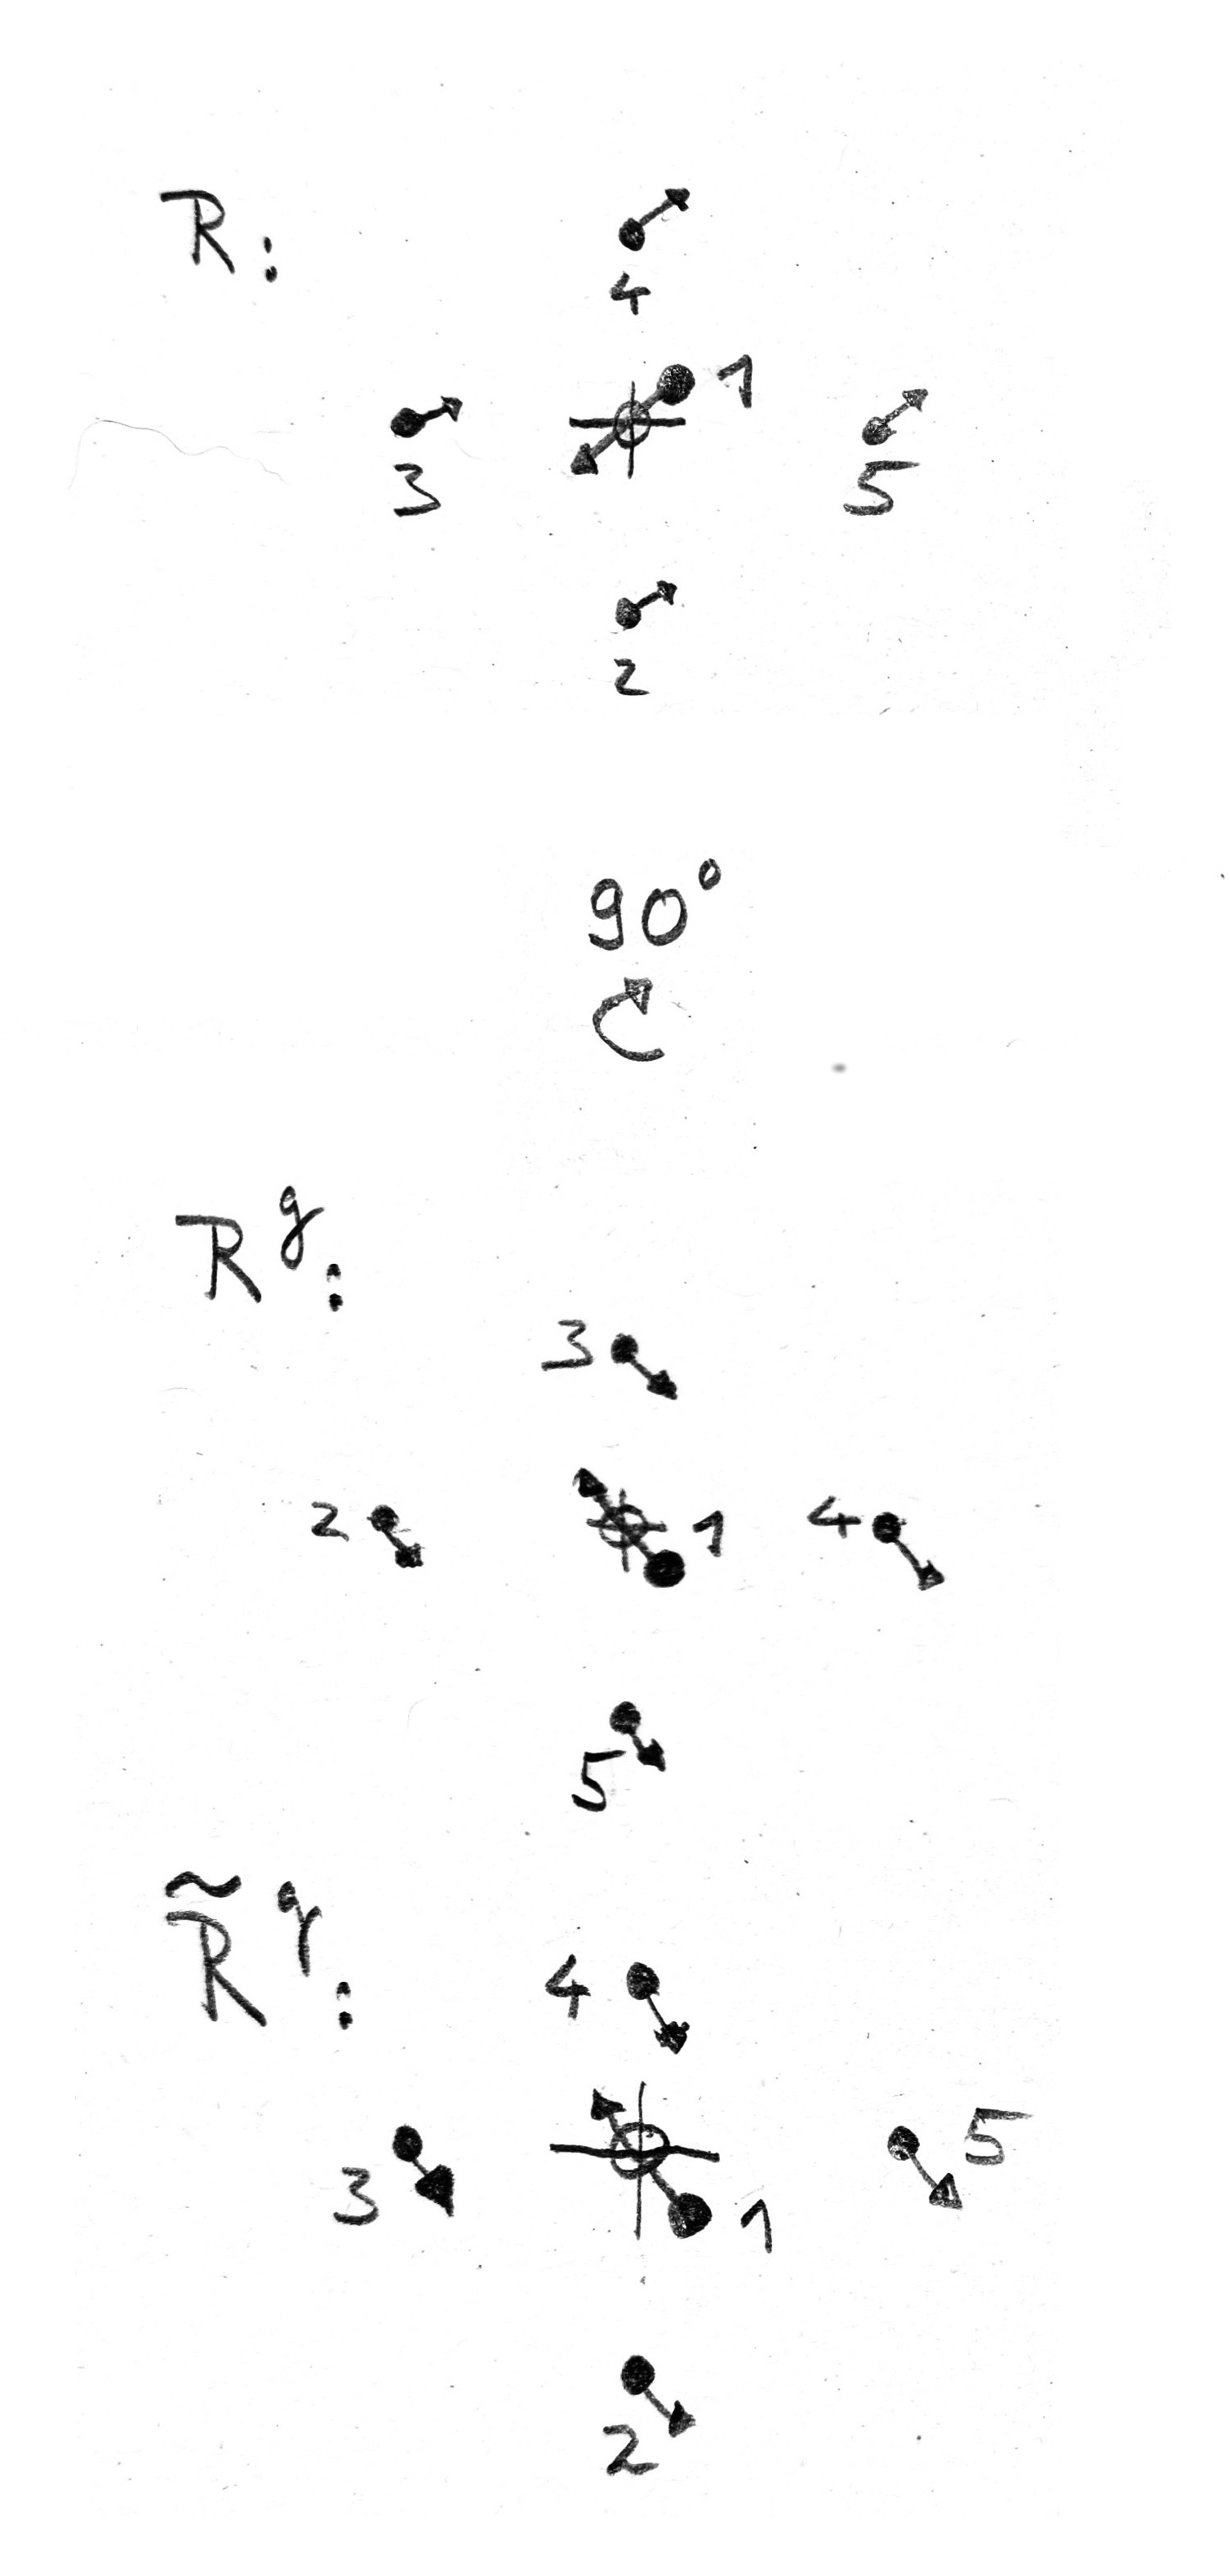
\includegraphics[width=\textwidth]{./sketches/symop.jpg}
  \caption{The configurations $\b R$, $\b R^g$, and $\tilde{\b R}^g$ obtained from the symmetry operation $g=\text{90 degrees rotation}$ for a two-dimensional system with five atoms. Arrows indicate the force at each atom.}
  \label{fig:symmetry.1}
\end{marginfigure}
As depicted in Fig.~\ref{fig:symmetry.1}, the forces on each atom in the rotated system $\b R^g = \set{\b R^g_I}$ are obtained by co-rotating the forces in the initial configuration $\b R = \set{\b R_I}$ as
\begin{align}
	\b F_I (\b R^g) &= {M}^g \b F_I (\b R)~,
	\label{eq:sym.Fp}
\end{align}
i.\,e.,~the forces transform as the displacements $\b U_I$. Let us now define a new configuration $\tilde{\b R}^g$ where just the displacements $\b U_I$ are rotated according to $g$. This can be achieved by rotating the entire system according Eq.\,\eqref{eq:sym.RI'} and applying the inverse permutation $P^{g-1}$,~i.\,e.,
\begin{align}
	\tilde{\b R}_I^g 
		&= P^{g-1}_{IJ} \b R_I^g 
		\stackrel{\eqref{eq:sym.RI'}}{=} \b R^0_I + {\rm M}^g P^{g-1}_{IJ} \b U_J~.
\end{align}
It follows that the force on atom $I$ in the new configuration $\tilde{\b R}^g$ is related to the force in the rotated system $\b R^g$ by this inverse permutation, so that
\begin{align}
		\b F_I (\tilde{\b R}^g) 
			&= {P}^{g-1}_{IJ} \b F_J (\b R^g) 
			= {M}^g  {P}^{g-1}_{IJ} \b F_J (\b R)~.
		\label{eq:sym.Ftilde}
\end{align}
By means of this equation, the set of forces obtained for a configuration $\set{\b R_I = \b R_I^0 + \b U_I}$ can be used to generate a set of forces for each symmetrically equivalent configuration $\set{\tilde{\b R}_I^g = \b R_I^0 + {\rm M}^g P^{g-1}_{IJ} \b U_J}$, where $g$ are spacegroup elements.

A complementary approach is to use the symmetry elements $\set{g}$ to reduce the forceconstant matrix to an irreducible basis,
\begin{align}
	\Phi 
		= \sum_{i=1}^{D} p_i \tilde{\Phi}_i~,
	\label{eq:sym.Phi.irrep.1}
\end{align}
where the $\tilde{\Phi}_i$ are \emph{solely} determined by the space group elements $\set{g}$ and analytical properties of the forceconstants, and only the \emph{irreducible components} $p_i$ are system dependent. The pseudoinverse procedure given in Eq.\,\eqref{eq:phi.pseudo.1} then only has to be performed for the $D$ parameters $p_i$~\cite{Parlinski1997}. This procedure can drastically reduce the number of free parameters in the forceconstant matrix. For example, in a $4\times4\times4$ bcc lattice with 128 atoms, $\Phi$ is a matrix with $(3 \cdot 128)^2 = 147456$ elements. However, there are only $D=11$ irreducible parameters $p_i$ that need to be determined~\cite{Hellman2013}.

\REM{Add the theory for symmetry reduction in practice to appendix?}

\newpage

\section{Geometry Optimization for Crystals}
\subsection{Lattice optimization at zero temperature}
\newthought{The task of geometry optimization} is to find a local minimum $\b R^0$ of the potential-energy surface $\mathcal{V} (\b R)$. From a mathematical point of view, $\mathcal V (\b R)$ is a function of the $3N$ coordinates $\b R$, or, when lattice degrees of freedom are included, $3N + 9$ degrees of freedom.\footnote{When rotations are rigorously excluded, the lattice only has 6~degrees of freedom.} Summarizing the positional degrees of freedom including the lattice in the generalized coordinate
\begin{align}
x 
= \left( R_{0}^x, R_{0}^y, \ldots, R_{N}^z; a^x_{~1}, a^x_{~2}, \ldots, a^z_{~3} \right) ~,
\label{eq:opt.x}
\end{align}
we seek to find
\begin{align}
x^0 = \arg \min_x \mathcal V (x)~.
\end{align}
The standard tools to solve this problem are very well covered in the standard reference~\cite{nocedal2006}. The technical pitfalls when optimizing lattices are thoroughly discussed in~\cite{pfrommer1997,Tadmor1999}.
A slightly different approach as the ones discussed in the references listed above is taken in the molecular simulations code \textsc{FHI-aims}~\cite{FHI-aims}. We therefore review this approach shortly in the following.

\newthought{Many optimization algorithms} working with gradients as input are based on the Newton descent method in which the target function is locally approximated by a second-order Taylor expansion~\cite{nocedal2006}. In our case, we denote the generalized force as $f_x$ and the Hessian matrix of second derivatives as ${\rm H}_{xx'}$, where
\begin{align}
f_x 
&= - \partial_x \mathcal V (x)~,
\label{eq:opt.f} \\
{\rm H}_{xx'} 
&= \partial_x \partial_{x'} \mathcal{V} (x)~.
\label{eq:opt.H}
\end{align}
Assuming that $f_x$ and ${\rm H}_{xx'}$ are known, the neighborhood of a configuration $x$ can be written to second order in a displacement $s_x$ as\marginnote{Sum convention \mbox{$s_x f_x \equiv \sum_x s_x f_x$} is implied.}
\begin{align}
m(x + s_x) 
= \mathcal V (x) - s_x f_x + \halb \fD s_x \fD {\rm H}_{xx'} \fP s_{x'}~.
\label{eq:opt.m}
\end{align}
The minimum of this function is given by
\begin{align}
s_x = {\rm H}_{xx'}^{-1} \fD f_{x'}~,
\end{align}
which is the essence of the Newton method. One beneficial property of the Newton method is that the exact Hessian $\rm H$ is not required to be known, and one can find approximate matrices $\rm B$ that yield good results. Replacing the exact $\rm H$ by an approximate matrix $\rm B$ is known as the \emph{quasi}-Newton method.
Typically, an initial approximate Hessian $\rm B^0$ is chosen to be of simple form,~e.\,g.,~a constant times unit matrix, or based on some simpler model~\cite{lindh1995}. The initial guess is then updated during the optimization, for example by means of the  Broyden–Fletcher–Goldfarb–Shanno (BFGS) algorithm.\footnote{BFGS update for the estimated Hessian $B^i$ from step $i$ to $i+1$:
	\begin{align*}
	{\rm B}^{i + 1}_{xx'}
	= {\rm B}^i_{xx'} 
	& + \frac{{\rm B}^i_{x\fP{y}} s^i_{\fP{y}} s^i_{y'} {\rm B}^i_{y'x'} }{s^i_{\fP y} {\rm B}^i_{yy'} s^i_{y'}}
	- \frac{\delta f^i_{\fP x} \delta f^i_{x'}}{\delta f^i_{\fP x} s^i_{x'}}~,
	\end{align*}
	with $\delta f^i = f^{i+1} - f^i$.
}
The configuration $x$ is updated according
\begin{align}
x^{i+1} = x^i + s_x^i = ~x^i + {\rm B}^i_{xx'} f^i_{x'}.
\end{align}

\newthought{If the lattice degrees of freedom} are represented by the Cartesian components $a^\alpha_i$ of the lattice vectors, the generalized force on the lattice is given by\marginnote{Symbolically:
	$$
	f_a 
	= -\frac{\partial \mathcal V}{\partial a} 
	= -V \underset{\fD \sigma}{\underbrace{\frac{1}{V}\frac{\partial \mathcal V}{\partial \varepsilon}}} \underset{\itp a}{\underbrace{\frac{\partial \varepsilon}{\partial a}}}~.
	$$
}
\begin{align}
f_a = - V \sigma \itp{a}~,
\end{align}
where $V = \det a$ is the unit cell volume, $\sigma$ is the $3 \times 3$~stress tensor, and $a$ is the lattice matrix.\footnote[][0em]{The lattice matrix is the collection of lattice vectors $\set{\b a_i}$,
	\begin{align}
	a = \begin{pmatrix} \b a_1, \b a_2, \b a_3 \end{pmatrix}~.
	\end{align}
}
For non-cubic systems, a diagonal Hessian matrix $B^0 = c \mathds 1$ will therefore produce steps proportional to the reciprocal cell $\itp{a}$ which, among other things, can break the space-group symmetry of the crystal. This behavior can be avoided by defining the initial Hessian as
\begin{align}
B^0 = c \itp{a} a^{-1}~,
\label{eq:opt.B0.new}
\end{align}
where $c$ is a numerical constant. This particular choice of $B^0$ can be viewed as making the Hessian diagonal in the native coordinate system of the lattice,~i.\,e.,~when deformations of the lattice are viewed as strain transformations in terms of the strain tensor $\varepsilon$. By the choice of the Hessian according to Eq.\,\eqref{eq:opt.B0.new}, the resulting steps $s^i_a$ will mimic such strain transformations early during the optimization:
\begin{align}
a^{i + 1} = a^i + s_a^i = (\mathds 1 + \varepsilon_s^i) a^i~.
\end{align}
Another detail that must be taken into account is that updates of the lattice necessarily have to keep the relative atomic positions expressed in the crystal basis,~i.\,e.,~their fractional coordinates, unchanged. The ideas outlined in this section have been implemented in~\textsc{FHI-aims} and the performance compared to the previous implementation is shown in Fig.\,\ref{fig:ltrm}.
\begin{marginfigure}
	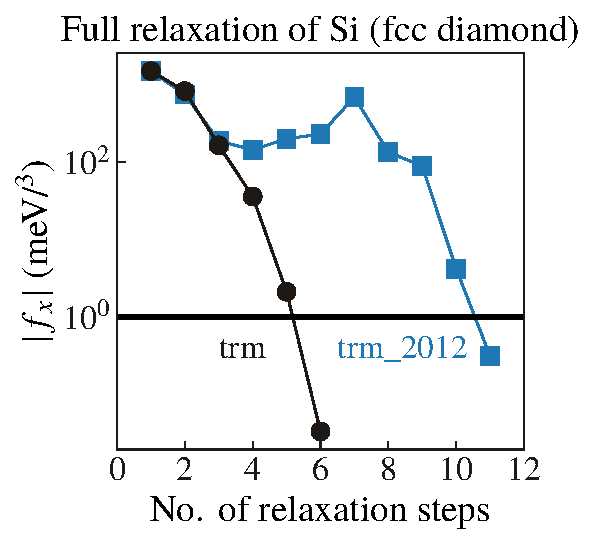
\includegraphics[width=\textwidth]{./plots/relaxation/ltrm.pdf}
	\caption{Residual force component as function of the relaxation steps, before (\texttt{trm\_2012}) and after (\texttt{trm}) optimizing the relaxation routine in \textsc{FHI-aims} according to the considerations presented in this chapter.}
	\label{fig:ltrm}
\end{marginfigure}
The non-systematic decrease of the residual force observed in the previous implementation (\texttt{trm\_2012}) was due to spurious distortions of the lattice and dislocations of the atomic arrangements generated by keeping their \emph{Cartesian} instead of \emph{fractional} positions unchanged during the lattice update. These artifacts are absent in the updated implementation (\texttt{trm}). The force convergence is generally faster and better behaved.


\subsection{Lattice optimization at finite temperature: Lattice expansion}
\newthought{At finite temperatures},\marginnote{The volume expansion is usually measured in terms of the \emph{thermal expansion coefficient} $\alpha (T)$~\cite{Kittel1969}
	\begin{align}
	\alpha (T) = \frac{1}{3 V} \frac{\partial V (T)}{\partial T}~.
	\label{eq:lattice.expansion.coefficient}
	\end{align}
}
the nuclear motion results in dynamical pressure $p(T)$ and the lattice reacts by deforming,
\begin{align}
a (T) = \bm ( \mathds 1 + \varepsilon (T) \bm ) a_0~,
\label{eq:lattice.T}
\end{align}
where $a_0$ is the 0\,K static lattice matrix, and $a (T)$ is the lattice at finite temperature given in terms of a \emph{strain transformation} $\varepsilon (T)$. 
The energy change per unit volume $\d W$ of a system subject to an infinitesimal strain deformation $\varepsilon$ is defined as
\begin{align}
\d W = \sigma_{\alpha}^{~\beta} \d \varepsilon^{\alpha}_{~\beta}~,
\label{eq:stress.strain}
\end{align}
where $\sigma$ is the \emph{stress tensor} of the system. The lattice $a(T)$ in thermal equilibrium will therefore be the lattice that minimizes the stress $\sigma$ in Eq.\,\eqref{eq:stress.strain}. Depending on the crystal symmetry~\cite{Nye1985}, the strain tensor $\varepsilon$ has up to six independent values. Equation\,\eqref{eq:stress.strain} therefore poses a six-dimensional optimization problem at a given temperature~$T$ which can be solved for example by coupling the system to a barostat and performing an $NPT$ simulation~\CITE{NPT}. In the language of the previous chapter, the lattice $a(T)$ is then given as a time or ensemble average $\braket{a}_{(p, T)}$ at thermodynamic conditions $(p, T)$. In practice however, this approach is quite inefficient and suffers from large noise, especially in the system sizes typically available to \emph{ab initio} MD simulations~\CITE{ai NPT}.

\newthought{An approximate solution} to the six-dimensional optimization problem of finding the finite temperature lattice $a (T)$ can be  found by the following rationale: We assume that the thermodynamic pressure at a given volume $V$ and temperature $T$ is given as
\begin{align}
p (V, T) \approx \frac{N k_{\rm B} T}{V} + p_{\rm pot} (V_0, T) + p_{\rm int}(V)~,
\label{eq:eos.p}
\end{align}
where $p_{\rm kin} (T) = N k_{\rm B} T / V$ is the kinetic pressure, and $p_{\rm pot} (V_0, T)$ is the potential part of the pressure in the system at reference volume $V_0$ which stems from the nuclear interaction $\mathcal V (\b R)$~\cite{Hansen1990}. The last term, $p_{\rm int} (V)$, is an internal pressure induced by the volume change. We assume that $p_{\rm int} (V)$ mainly stems from the lattice and is not temperature dependent. It can therefore be obtained from an equation of state parametrized at 0\,K, for example the \emph{Vinet equation}~\cite{Vinet1987}:
\begin{align}
p_{\rm int} (V) 
&= \frac{3 B_0}{X^2} (1-X) {\rm e}^{\eta (1-X)} \label{eq:p.Vinet} \quad\text{with} \\ 
X &= \left[\frac{V}{V_0}\right]^{\frac{1}{3}}
\quad\text{and}\quad
\eta 
= \frac{3}{2} \left(B_0' - 1 \right)~,
\end{align}
where $V_0$ is the volume, $B_0$ is the bulk modulus, and $B_0' = \partial B_0 / \partial p$ is the isothermal pressure derivative of the bulk modulus. All these three parameters are obtained for the static lattice and we neglect their temperature dependence. Once the full parametrization of Eq.\,\eqref{eq:eos.p} is known, the temperature-dependent volume $V_{\rm min} (T)$ is found by requiring zero pressure. The resulting pressure $p_{\rm int} (V_{\rm min})$ can be used to find the static reference lattice $a(T)$ by optimizing the geometry while applying the external pressure $p_{\rm relax} = - p_{\rm int} (V_{\rm min})$ as depicted in Fig.\,\ref{fig:lattice.expansion}.
\begin{marginfigure}
	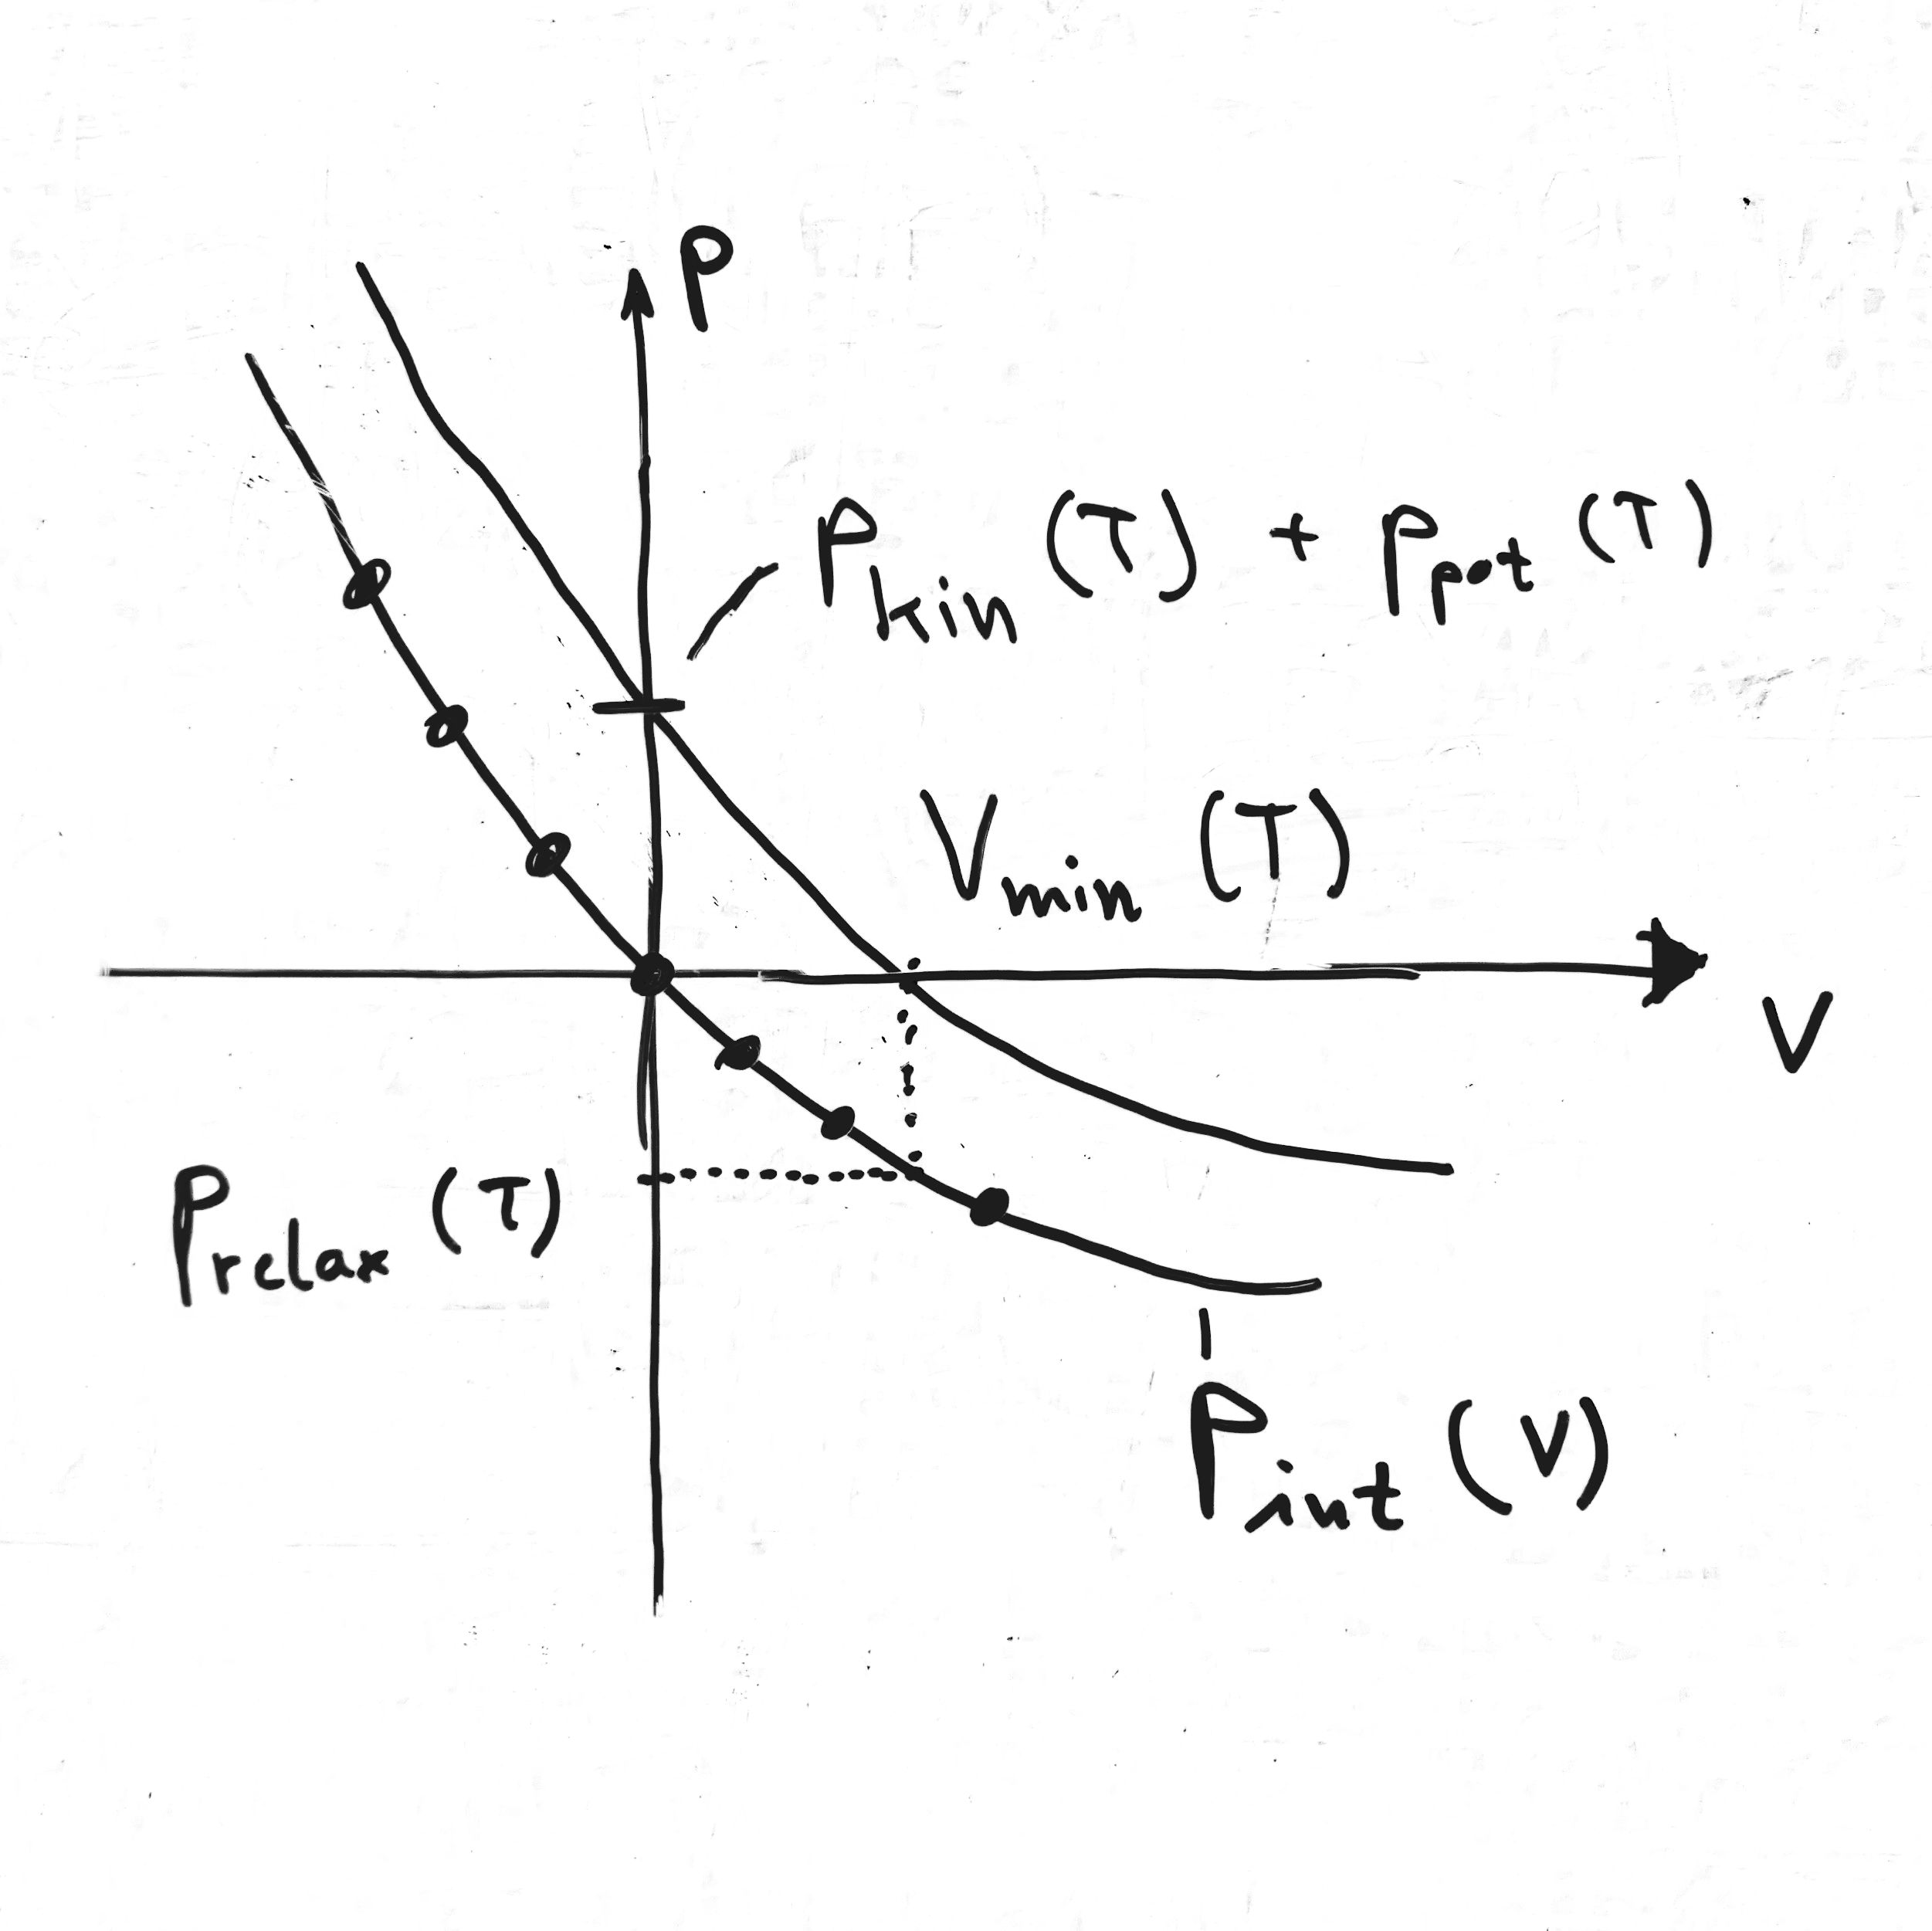
\includegraphics[width=\textwidth]{./sketches/lattice_expansion.jpg}
	\caption{Determination of relaxation pressure to obtain lattice at finite temperature. Dots denote volumes used to parametrize Eq.\,\eqref{eq:p.Vinet}.}
	\label{fig:lattice.expansion}
\end{marginfigure}
The lattice $a (T)$ obtained this way will then generate the static pressure contribution $p_{\rm int}$ which compensates the dynamical contributions stemming from kinetic and potential energy.

\newthought{The procedure goes as follows}:
\begin{enumerate}
	\item To parametrize $p_{\rm int} (V)$, calculate a $p(V)$ curve for different volumes\footnote{For non-cubic systems or systems with internal degrees of freedom, use a set of external pressures $p_{\rm relax}$ to obtain a set of reference structures at different volumes $V_{p_{\rm relax}}$ by geometry optimization.} and fit the Vinet equation of state given by Eq.\,\eqref{eq:p.Vinet} to obtain $(V_0, B_0, B_0')$.
	\item Perform MD simulation at $V_0$ and target temperature $T$ until pressure $p_{\rm pot} (V_0, T)$ is sufficiently  converged.
	\item Minimize Eq.\,\eqref{eq:eos.p} with respect to volume to find $V_{\rm min} = \arg \min_V p (V, T)$.
	\item Predict pressure $p_{\rm relax} = - p_{\rm int} (V_{\rm min})$ and obtain a reference structure of correct volume $V_{\rm min}$ by applying this pressure during a geometry optimization, see Fig.\,\ref{fig:lattice.expansion}. The lattice of this structure will satisfy $\det a(T) = V_{\rm min}$.
\end{enumerate}

\newthought{After the lattice $a (T)$ is obtained}, it should be verified that the pressure $p (V_{\rm min}, T)$ is indeed minimized. If a significant residual pressure $p_{\rm residual}$ persists it can be added to the pressure used for relaxation until self consistence is reached.

\newpage

\section{Statistical Mechanics and Molecular Dynamics}
There exist plenty of excellent books on statistical mechanics, some of which are included in the references~\cite{Phillies2012,Tuckerman,Schrodinger1989}. This chapter merely serves to recall the most important notions necessary for computing properties of materials under thermodynamic conditions, and introduce the notation used in the following remainder of the work. In particular, the concepts of \emph{ensemble}, \emph{state}, and \emph{averages} are briefly introduced.

\newthought{A thermodynamic \emph{ensemble}} can be viewed as a complete list of all allowed \emph{states} $\Gamma$ of a system of particles, where the state is an instantaneous snapshot of all microscopic variables~\cite{Phillies2012}. In classical statistical mechanics, these variables are the positions~$\b R$ and momenta~$\b P$. A particular configuration $\Gamma = \set{\b R, \b P}$ is called \emph{phase-space point}, and the phase space is the collection of all points $\Gamma$ compliant with external constraints.\footnote{Easiest example of an external constraint: If the particles are confined in a box with impenetrable walls, the possible position $\b R$ are necessarily confined to that box. Other constraints comprise total energy, particle number, and more.} To each state $\Gamma$, a statistical weight $f (\Gamma)$ is assigned, where $f$ is called the \emph{distribution function}. A thermodynamic ensemble is completely specified by the set of external constraints under which the mechanical system evolves, and the associated statistical weight function $f$.

\newthought{Statistical averages of phase-space functions} can be obtained by averaging over all permissible states $\Gamma$ with the statistical weight given by the distribution function, $f (\Gamma)$. The \emph{phase-space average} of a generic phase-space function $A (\Gamma)$ is defined as
\begin{align}
  \braket{A}_f 
    = \int \d \Gamma ~ A(\Gamma) f (\Gamma)~.
  \label{eq:phase.space.average}
\end{align}

An alternative approach towards computing averages is the concept of time averaging. The \emph{time average} of a phase-space function is defined as
\begin{align}
  \braket{A}_t
    = \lim\limits_{t \to \infty} \frac{1}{t} \int_0^t \d t' ~ A {\bm (} \Gamma(t') {\bm )}~.
  \label{eq:time.average}
\end{align}
A system for which the phase-space and the time average are identical is said to be \emph{ergodic}. The \emph{ergodic hypothesis} states that this is true for most systems with non-pathological particle interaction $\mathcal V$. Albeit being virtually impossible to prove rigorously, this hypothesis is the underlying idea of \emph{molecular dynamics} (MD) simulations, where the statistical behavior of a system is assessed by choosing a suitable initial condition and propagating it in time by numerically solving the equations of motion.

\newthought{In this work}, we use two thermodynamic ensembles: the microcanonical, $NVE$ for short, where the total energy $E$ of the system is conserved, and the canonical ($NVT$), where the system can be viewed as coupled to a bath of temperature $T$. The latter is mimicking more realistic experimental conditions, where usually the temperature and not the total energy of the system can be controlled. Technically, experiments are performed rather at constants pressure $p$ instead of constant volume, and the correct ensemble to describe such a situation is the isothermal-isobaric one commonly denoted as $NPT$. In practice however, the canonical ensemble is easier to simulate and is a good approximation to the $NPT$ ensemble when the system size is not too small~\cite[p.\,134]{Tuckerman}


\subsection{Microcanonical Ensemble}
The microcanonical ensemble is characterized by three conserved extensive quantities: particle number $N$, system volume $V$, and total energy $E$. The total energy of a given microstate,~i.\,e.,~the configuration of particles and their momenta represented by the phase-space point $\Gamma = \set{\b R, \b P}$, is given by the Hamiltonian of the system, $H (\Gamma)$. 
%The central postulate of statistical mechanics is that each microstate is equally probable. Therefore, any point in phase space $\Gamma$ yielding an energy in a thin interval around the target energy, $H (\Gamma) \in [E, E + \d E]$, is realized with the same likelihood. Taking particle number $N$ and system volume $V$ to be fixed and non-controllable, the expectation value of a phase-space observable $A$ in an ensemble of energy $E$ is defined as
%\begin{align}
%	\braket{A}_E 
%		= \int \d \Gamma ~ A(\Gamma) f_E (\Gamma)~.
%	\label{eq:phase.space.expectation}
%\end{align}
%Here, the \emph{microcanonical distribution function} $f_E$ is enforcing that phase-space points are sampled with equal probability which is achieved by defining
% \newthought{The microcanonical distribution function} is defined as
The microcanonical distribution function is defined as
\begin{align}
f_E (\Gamma) = \frac{1}{\mathcal{Z}_E} \delta {\bm (} H (\Gamma) - E {\bm )}~,
\end{align}
where the microcanonical partition sum $\mathcal{Z}_E$ is a normalizing factor for $f_E$. The partition function $f_E$ encapsulates the underlying postulate of the microcanonical ensemble,~i.\,e.,~that any point in phase space $\Gamma$ yielding an energy $H (\Gamma)$ in a thin interval around the target energy $E$ 
%, $H (\Gamma) \in [E, E + \d E]$, 
will be realized with the same likelihood.

\newthought{The time evolution of a system} is governed by the Hamiltonian which generates an energy conserving propagation of a phase space point $\Gamma (t) = \set{\b R (t), \b P (t)}$ in terms of Hamilton's equations,
\begin{align}
	\dot{\b R}_I (t) = \frac{\partial H}{\partial \b P_I} \quad\text{and}\quad
	\dot{\b P}_I (t) = -\frac{\partial H}{\partial \b R_I}~.
	\label{eq:stat.eom}
\end{align}
The temporal evolution of an observable $B$ is then given by the Liouville equation~\cite{Tuckerman}
\begin{align}
	\dot{B} = \set{B, H} \equiv \im L B~,
	\label{eq:Liouville}
\end{align}
where $L$ is the \emph{Liouville operator} defined by its action according to Eq.\,\eqref{eq:Liouville}, and $\set{\cdot , \cdot}$ denotes the \emph{Poisson bracket}.\marginnote{
The Poisson bracket is defined by
\begin{align}
	\set{B, H}
		= \sum_{I, \alpha} \frac{\partial B}{\partial R_I^\alpha} \frac{\partial H}{\partial P_I^\alpha}
			- \frac{\partial B}{\partial P_I^\alpha} \frac{\partial H}{\partial R_I^\alpha}
%		= \sum_{I, \alpha} \frac{\partial B}{\partial R_I^\alpha} \dot{R}_I^\alpha
%			+ \frac{\partial B}{\partial P_I^\alpha} \dot{P}_I^\alpha~.
	\label{eq:Poisson}
\end{align}
}
The Liouville equation is formally solved by
\begin{align}
	B (t) = {\rm e}^{\im L t} B(0)~,
	\label{eq:B.time.evolution}
\end{align}
the operator ${\rm e}^{\im L t}$ is therefore called the \emph{time evolution operator} or \emph{classical propagator}.
%\paragraph{Ergodic hypothesis}
%Under the assumption that a system initially prepared in a configuration with correct energy dynamically evolves through the entire permissible phase space, the phase-space average defined in Eq.\,\eqref{eq:phase.space.expectation} can be written in terms of a \emph{time average} defined as
%\begin{align}
%  \braket{A}_E 
%    = \left. \lim\limits_{t \to \infty} \frac{1}{t} \int_0^t \d t' ~ A {\bm (} \Gamma(t') {\bm )}
%	    \right\vert_{H \bm ( \Gamma (0) \bm ) = E}~.
%	\label{eq:time.average}
%\end{align}
%A system for which the phase-space and the time average are identical is said to be \emph{ergodic}. The \emph{ergodic hypothesis} states that this is true for most systems with non-pathological interaction $V$. Albeit being virtually impossible to prove rigorously, this hypothesis is underlying idea of \emph{molecular dynamics} (MD) simulations, where the statistical behavior of a system is assessed by choosing a suitable initial condition and propagating it in time via the classical equations of motion given by Eq.\,\eqref{eq:stat.eom}.
In practice, the equations of motion are solved numerically, for example by the \emph{velocity Verlet} algorithm~\CITE{Verlet1967,Swope1982},
\begin{subequations}
\begin{align}
	\b R_I (t + \delta t) 
		&= \b R_I (t) + \delta t \dot{\b R}_I (t) + \frac{\delta t^2}{2 M_I} \b F_I(t) + \mathcal{O} (\delta t^4)~, \\
	\dot{\b R}_I (t + \delta t) 
		&= \dot{\b R}_I (t) + \frac{\delta t}{2 M_I} \left[\b F_I(t) + \b F_I (t + \delta t)\right] + \mathcal{O} (\delta t^4)~.
\end{align}
\label{eq:VelocityVerlet}
\end{subequations}
The velocity Verlet algorithm introduces an error of order $\delta t^4$ in the integration step, but has two important properties mitigating a negative impact on obervables: First, a velocity Verlet integration step is time-reversible, an important prerequisite for long-term stability of the total energy for symmetry reasons. Second, the velocity Verlet map from $t$ to $t + \delta t$ has the property of being \emph{symplectic}~\cite[p.\,101]{Tuckerman}. This means that the discrete time propagation is not guaranteed to preserve the energy along the trajectory $\Gamma(t)$, but there exists a Hamiltonian $\tilde{H} (\Gamma, \delta t)$ which is conserved exactly and fulfills $\tilde{H (\Gamma, \delta t)} \to H(\Gamma)$ for vanishing timestep $\delta t \to 0$~\cite[p.\,121]{Tuckerman}. The symplectic property is formalized in the ``shadowing theorem'', which states that existence of a ``shadow Hamiltonian'' $\tilde H$ ensures that errors introduced by using a finite time step are bounded~\CITE{see tuckerman}.

\subsection{Canonical ensemble}
The canonical ensemble is characterized by the two extensive variables particle number $N$ and volume $V$, and the intensive quantity temperature $T$. It can be viewed as representing a system in contact with an infinite thermal bath of temperature $T$, where heat can be exchanged via a weak coupling.

In analogy to the previous section, we define the \emph{canonical distribution function} at inverse temperature $\beta = 1 / k_{\rm B} T$
\begin{align}
	f_\beta (\Gamma) 
		= \frac{1}{\mathcal{Z}} {\rm e}^{- \beta H (\Gamma)}~,
	\label{eq:f.canonical}
\end{align}
where the  canonical partition sum $\mathcal{Z}$ normalizes $f_\beta$. 
%The canonical expectation value is therefore given by
%\begin{align}
%	\braket{A}_\beta = \int \d \Gamma ~ A(\Gamma) f_\beta(\Gamma)~.
%\end{align}

\newthought{As we have seen earlier}, a time-independent Hamiltonian generates energy-preserving dynamics via the equations of motion given in Eq.\,\eqref{eq:stat.eom}. To perform a simulation at non-constant energy, the coupling to a thermal bath therefore has to be incorporated explicitly into the equations of motion. One of the many ways to achieve this is via the \emph{Langevin equation}~\cite{Vanden2006} in which the change of momentum is modified,
\marginnote{
	% \normalsize
	The stochastic force is given by:
	\begin{align*}
	\b F^{\rm stochastic}_I (t) 
	&= \sqrt{2 k_{\rm B} T M_I \gamma} \eta (t)~, \\
	\braket{\eta (t) \eta (0)}
	& = \delta (t)~.
	\end{align*}
	It replenishes the kinetic energy dissipated by the friction proportinoal to $\gamma$, see discussion in Ref.\,\cite[p.\,328]{Phillies2012}.
}
\begin{align}
	\dot{\b P}_I (t) 
		&= \b F_I (t) - \gamma \b P_I (t) + \b F^{\rm stochastic}_I (t)~.
	\label{eq:stat.Langevin}
\end{align}
This equation describes a perturbation of the nuclei induced by a velocity-dependent friction proportional to a constant $\gamma$,%\marginnote{From Eq.\,\eqref{eq:stat.Langevin} follows that $\gamma$ has the unit of inverse time.}
and a stochastic force proportional to a white-noise kernel $\eta (t)$. With the modified equation of motion in terms of the stochastic force, an ergodic time evolution that generates the canonical distribution can be obtained, so that
\begin{align}
  \braket{A}_t = \braket{A}_{f_\beta}~.
\end{align}
%hypothesis for the canonical ensemble can be stated,
%% 
%\begin{align}
%	\braket{A}_\beta
%		= \left. \lim\limits_{t \to \infty} \frac{1}{t} \int_0^t \d t' ~ A {\bm (} \Gamma(t') {\bm )}
%			\right.~,
%	\label{eq:time.average.canonical}
%\end{align}
%where the time evolution of the system is given by Eq.\,\eqref{eq:stat.Langevin} and the friction constant is chosen such that the expectation value $\braket{A}_\beta$ is insensitive to the chosen value.

\REM{The Langevin equation can be used to thermalize a system and generate a canonical ensemble starting from some initial configuration $\b R^0$} \cite[p.\,590]{Tuckerman}
\REM{Plot: Temperature evolution and velocity distribution.}


\TODO{Other approaches: Nose-Hoover, Berendsen vr, svr, ...}
\TODO{Some plots}